% Plain-language review document (explaneat plain-language review), v5.
\documentclass[a4paper,10pt]{article}
\usepackage[margin=1.8cm]{geometry}
\usepackage{amsmath}
\usepackage{amssymb}
\usepackage{booktabs}
\usepackage{tabularx}
\usepackage{graphicx}
\usepackage[table,usenames,dvipsnames]{xcolor}
\usepackage{tikz}
\usetikzlibrary{arrows.meta,fit,backgrounds,positioning,calc}
\usetikzlibrary{shapes.geometric}
\usepackage{longtable}
\usepackage{pdflscape}
\usepackage{float}
\usepackage[font=small,labelfont=bf]{caption}
\usepackage{array}
\usepackage[unicode=true,hidelinks]{hyperref}
\setcounter{tocdepth}{3}
\setcounter{secnumdepth}{3}
% Review markers, copied from dissertation.tex (7 Nov 2026) for standalone builds.
\newif\ifreviewmarks
\reviewmarkstrue
\newcommand{\reviewrule}{\noindent{\color{BrickRed}\rule{\linewidth}{0.8pt}}}
\newenvironment{drafted}[1][]{%
  \ifreviewmarks\par\addvspace{\medskipamount}\reviewrule\par\nopagebreak
  \noindent{\color{BrickRed}\sffamily\footnotesize\textbf{Thesis Draft}\quad #1\hfill review}\par\nopagebreak\smallskip\fi}{%
  \ifreviewmarks\par\smallskip\noindent{\color{BrickRed}\sffamily\footnotesize end of thesis draft}\par\nopagebreak\reviewrule\par\medskip\fi}
\newcommand{\figreview}[1]{\ifreviewmarks\par\smallskip{\color{NavyBlue}\sffamily\footnotesize\textbf{Figure note:} #1}\par\fi}
\begin{document}
\begin{center}{\Large\bfseries Plain-language explanation: heart-s5-c1\par}\vspace{2mm}{\small AI-assisted drafts for review. Nothing here has been verified by a person.\par}\end{center}
\noindent\textbf{How to read this.} Explanations are built up but read down: the summary first, then each part from the whole model down, in plain words, each sentence followed by the claims it rests on (C01, C02, \ldots; every cited claim was computed on the model and checked). Numbers are changes in predicted risk for a typical patient. The technical record (original hypotheses, formulas, evidence tables with the test check, ranges and n) is at the end. The text describes what the model does, not the world; whether it is plausible is for the reviewer to judge.
\par\medskip\noindent\textbf{What changed in v5e (figures).} v5e: every diagram is a numbered figure with a caption (list of figures after the contents) and the text refers to it; the whole-network figure has its own landscape page, scaled to the page, with a short caption and its description in the text; an input used by several parts is drawn under each of them (same input, repeated for readability, dotted outline); and an appendix figure shows the trained network before any explanation (no parts, no splits).
\par\medskip\noindent\textbf{What changed in v5c (tables and diagrams).} v5c: the evidence tables are landscape, compact and shaded by row, with the header repeated on every page (longtable and pdflscape, used in this review PDF only; the thesis preamble has neither). In the diagrams each input is drawn once, in a shared row along the bottom (the explanation's split copies of an input are listed in the technical detail instead), every cluster has one output rectangle with its plain name, the inputs that feed the output directly meet in a drawn 'sum', and a one-line legend explains the edges.
\par\medskip\noindent\textbf{What changed in v5b (diagrams).} v5b uses one grouping everywhere, the annotation hierarchy: the summary's diagram is the same picture as the whole model's section, and a part that is itself a weighted sum (blood pressure with cholesterol) is a part of its own, described as one that adds up, so the text counts three parts throughout; the lint checks every 'N parts' against the hierarchy. A full-structure diagram follows the summary: every node and connection, nested by part, with the inputs that feed the output directly in their own cluster and the unused input columns listed. Each section from the top down adds its own region of that diagram, with stubs for connections from or to other parts; each connection is drawn in exactly one section. The gate's text now says that it lowers the risk for the patients it acts on, and that more vessels and higher cholesterol take that lowering away; its vessel statements are one per group.
\par\medskip\noindent\textbf{What changed in v5 (read down).} v5 reads the explanation down. The summary (one line, a diagram, one paragraph per block) is as in v4, except that the paragraph on what adds up is split into protective items, risk-raising items and rare results, and an input that also feeds a part is quoted with its direct contribution only (the rest is in that part's paragraph). Then the document walks the annotation hierarchy from the whole model down: for each part a plain hypothesis (what it does for the prediction), plain evidence (what was checked and what it showed; for a part made of others, what they are and how they combine), a diagram one level down and where to read on. The original hypotheses, closed forms and evidence tables are in 'Technical detail' at the end. Statements about structure (what a part is made of, a copy of another part, a formula that reproduces it) are now claims of their own, checked on the graph and the data.
\par\medskip\noindent\textbf{v4.} v4 follows the structure of the explanation. The summary opens with one line and a diagram at the same grouping, then gives one paragraph per top-level block of the annotation hierarchy: one for everything that adds up independently (the inputs that feed the model score directly, and parts that are a weighted sum), and one for each part that combines its inputs in another way: what it combines, how, and for whom. 'Parts in detail' follows the hierarchy below that, with a diagram one level down for each part that contains others. The prose no longer says 'clearly', 'slightly', 'consistently' or 'on the training data only': the numbers carry it, and the test check, the ranges and n stay in the evidence tables. Only genuinely small groups are marked, with their n. The lint rejects the confidence words and checks the block structure.
\tableofcontents
\listoffigures
\clearpage
\begin{drafted}[plain-language layer: heart-s5-c1]
\section{heart-s5-c1}
\noindent{\small Genome \texttt{4f9f15fb-446b-4560-9704-c7b1a83617b5}, explanation \texttt{39c7fe21-518b-4517-8765-7e6008dc7d98}. Split: train primary (n=242), test as a check (n=61). Claims: 52, verified 48, not supported 4.\par}
\noindent{\small\textcolor{BrickRed}{AI-assisted draft for review (unverified)}\par}\smallskip
\noindent{\footnotesize Reference (typical) patient: the typical patient: the median training patient for every number and the most common training category for every category (not a real patient). age: 56 years; ca: 0 vessels; chol: 240 mg/dL (6.2 mmol/L); cp: no chest pain (asymptomatic); exang: no chest pain on exercise; fbs: fasting blood sugar of 120 mg/dL or less; oldpeak: 0.8 mm; restecg: a normal resting ECG; sex: male; slope: an upsloping ST segment; thal: a normal thallium scan; thalach: 152 beats per minute; trestbps: 130 mm Hg. Predicted risk of heart disease: 22\%.\par}
\subsection{Summary}
\noindent For a typical patient (a 56-year-old man with no chest pain symptoms and median test results) the model predicts a risk of heart disease of about 22\%; it adds up most of its inputs independently, and a chain of three parts adds to that sum: a signal from ST depression on exercise, the thallium scan and the resting ECG that acts on 116 of 242 training patients, a blood pressure step that reads that signal, and an extra age term that acts on 85 patients.\,{\scriptsize\textcolor{NavyBlue}{[C32, C40, C51]}} Figure~\ref{fig:hearts5c1:summary} shows the model at this level: one box per paragraph below.
\par\medskip\noindent\fbox{\begin{minipage}{0.96\linewidth}\small\textbf{How to read the diagrams.} Edge colour is the sign of that one connection: blue positive, red negative; thicker is a larger weight. The outline and arrow on an input (and on a part's output box) is its overall effect on the final prediction, read from the verified claims: orange and up arrow raises it, teal and down arrow lowers it, grey and double arrow depends (it goes both ways, or differs between levels). A negative connection into a part that itself raises the prediction means that input lowers the prediction; through a hinge the overall effect can only be read from the claims, not from the edges. Up arrow means towards heart disease; down arrow, away from it. A double outline marks an input (or a part's output) that acts at a fixed rate everywhere: it adds the same amount to the score per unit, so it is explained by its rate alone (see 'Linear factors'); a dashed double outline, at a fixed rate on the observed data. The normal outline is an input whose effect switches on and off somewhere. For example, age has a positive connection into 'Extra age term', a part that raises the predicted risk of heart disease, so age raises it.\end{minipage}}\par\medskip
\begin{figure}[H]\centering
\resizebox{!}{\ifdim\height>0.5\textheight 0.5\textheight\else\height\fi}{%
\resizebox{\ifdim\width>\linewidth\linewidth\else\width\fi}{!}{%
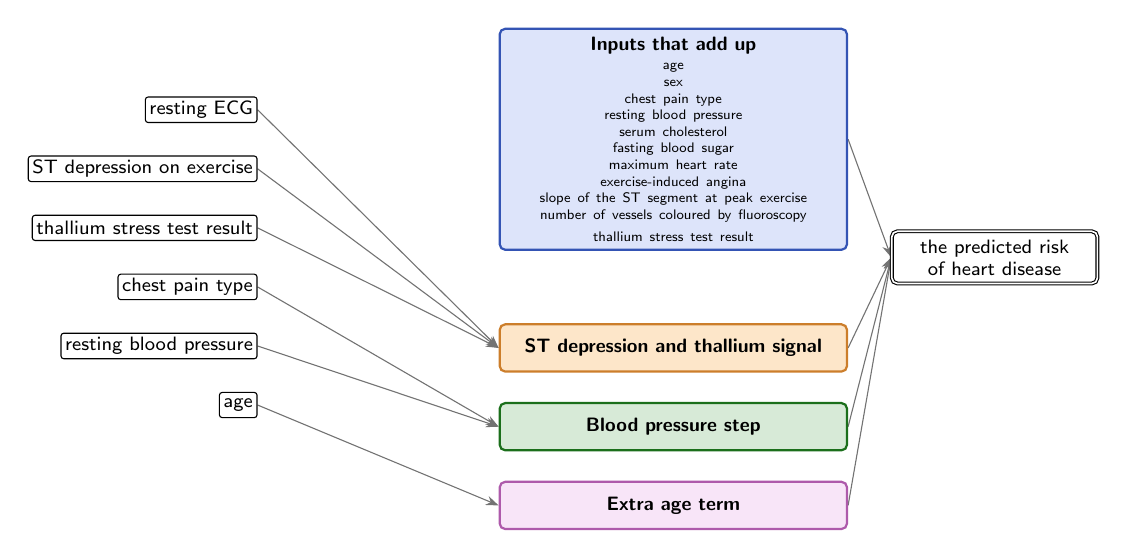
\begin{tikzpicture}[
  font=\sffamily\scriptsize, >={Stealth[length=1.6mm]},
  inp/.style={draw, rounded corners=1pt, fill=white, inner sep=1.5pt, minimum height=3.2mm, anchor=east},
  abox/.style={draw, thick, rounded corners=2pt, align=center, inner sep=3pt, minimum height=6mm, text width=42mm},
  outp/.style={draw, double, rounded corners=2pt, fill=white, align=center, inner sep=3pt, text width=24mm},
  agg/.style={draw=black!55},
]
\node[inp] (i0) at (0,1.875) {resting ECG};
\node[inp] (i1) at (0,1.125) {ST depression on exercise};
\node[inp] (i2) at (0,0.375) {thallium stress test result};
\node[inp] (i3) at (0,-0.375) {chest pain type};
\node[inp] (i4) at (0,-1.125) {resting blood pressure};
\node[inp] (i5) at (0,-1.875) {age};
\node[abox, fill=RoyalBlue!18, draw=RoyalBlue!80!black] (b0) at (5.28,1.5) {\textbf{Inputs that add up}\\[1pt]{\tiny age\\ sex\\ chest pain type\\ resting blood pressure\\ serum cholesterol\\ fasting blood sugar\\ maximum heart rate\\ exercise-induced angina\\ slope of the ST segment at peak exercise\\ number of vessels coloured by fluoroscopy\\ thallium stress test result}};
\node[abox, fill=BurntOrange!18, draw=BurntOrange!80!black] (b1) at (5.28,-1.15) {\textbf{ST depression and thallium signal}};
\node[abox, fill=ForestGreen!18, draw=ForestGreen!80!black] (b2) at (5.28,-2.15) {\textbf{Blood pressure step}};
\node[abox, fill=Orchid!18, draw=Orchid!80!black] (b3) at (5.28,-3.15) {\textbf{Extra age term}};
\node[outp] (out) at (9.36,0) {the predicted risk of heart disease};
\begin{scope}[on background layer]
\draw[->, agg] (b0.east) -- (out.west);
\draw[->, agg, thin] (i0.east) -- (b1.west);
\draw[->, agg, thin] (i1.east) -- (b1.west);
\draw[->, agg, thin] (i2.east) -- (b1.west);
\draw[->, agg] (b1.east) -- (out.west);
\draw[->, agg, thin] (i3.east) -- (b2.west);
\draw[->, agg, thin] (i4.east) -- (b2.west);
\draw[->, agg] (b2.east) -- (out.west);
\draw[->, agg, thin] (i5.east) -- (b3.west);
\draw[->, agg] (b3.east) -- (out.west);
\end{scope}
\end{tikzpicture}}}%
\caption{The model at the level of the summary: one box per part.}
\label{fig:hearts5c1:summary}
\end{figure}
\paragraph{Inputs that add up.} \par\noindent\textit{Lowering the risk.}  These add up independently, and these lower the risk: being a woman takes a typical patient's predicted risk from about 22\% to about 3\% and fasting blood sugar above 120 mg/dL to about 11\%; a higher maximum heart rate lowers it steadily, from about 27\% at 118 to about 18\% at 175 beats per minute; and through this sum alone typical angina lowers it to about 2\%, non-anginal chest pain to about 5\% and atypical angina to about 11\% (chest pain type also acts through the blood pressure step, below).\,{\scriptsize\textcolor{NavyBlue}{[C12, C17, C22, C10, C13, C20]}} \par\noindent\textit{Raising the risk.}  Each extra vessel coloured by fluoroscopy adds about the same, from about 22\% at 0 to about 88\% at 2 vessels, flattening out near the top because the predicted risk cannot go much higher; a flat rather than upsloping ST segment raises it to about 67\%, higher cholesterol raises it steadily from about 14\% at 193 mg/dL to about 37\% at 308 mg/dL, and chest pain brought on by exercise raises it to about 33\%.\,{\scriptsize\textcolor{NavyBlue}{[C01, C04, C07, C16]}} Through this sum alone, higher resting blood pressure raises it steadily, from about 14\% at 110 mm Hg to about 35\% at 155 mm Hg, older age raises it steadily, from about 19\% at 42 to about 24\% at 66 years, and a reversible defect on the thallium scan raises it to about 35\%; all three also act through the parts below.\,{\scriptsize\textcolor{NavyBlue}{[C08, C24, C15]}} \par\noindent\textit{Rare results.}  Some rarer results also count (the model has little data on this, n = 2 to 17): through this sum alone a thallium result coded 4 raises the risk to about 83\% and a fixed defect on the thallium scan lowers it to about 11\%, and a downsloping ST segment raises it to about 27\%.\,{\scriptsize\textcolor{NavyBlue}{[C02, C18, C25]}}
\paragraph{ST depression and thallium signal.} This part reads ST depression on exercise, the thallium scan and the resting ECG, and acts on 116 of 242 training patients, 77 of whom had heart disease; for the typical patient it acts on, the predicted risk is about 89\% without it and about 96\% with it.\,{\scriptsize\textcolor{NavyBlue}{[C40]}} Through it, more ST depression adds to the predicted risk only once it rises above about 0.9 mm, rising in an uneven way: for a typical patient from about 22\% at 0 mm to about 48\% at 2.8 mm.\,{\scriptsize\textcolor{NavyBlue}{[C33, C39]}} ST depression counts more with a reversible defect on the thallium scan (from about 36\% to about 80\%, against about 22\% to about 48\% otherwise) and with a normal resting ECG (from about 22\% to about 48\%, against about 22\% to about 34\% otherwise), in an uneven way.\,{\scriptsize\textcolor{NavyBlue}{[C36, C37]}} A reversible defect on the thallium scan also raises the risk more with a normal resting ECG, from about 22\% to about 47\% against about 22\% to about 36\% otherwise.\,{\scriptsize\textcolor{NavyBlue}{[C38]}}
\paragraph{Blood pressure step.} This part reads that signal together with resting blood pressure and chest pain type, and barely changes the predictions: for the typical patient it acts on, atypical angina raises the predicted risk through it from about 69\% to about 70\%, and non-anginal chest pain leaves it at about 69\%.\,{\scriptsize\textcolor{NavyBlue}{[C42, C44]}}
\paragraph{Extra age term.} This part acts on 85 of 242 training patients, 37 of whom had heart disease; for the typical patient it acts on, the predicted risk is about 28\% without it and about 30\% with it.\,{\scriptsize\textcolor{NavyBlue}{[C51]}} Through it, age adds nothing until about 53 years (between 53 and 66 years for different patients), then raises the risk steadily, for a typical patient from about 21\% at 42 to about 24\% at 66 years.\,{\scriptsize\textcolor{NavyBlue}{[C49, C50]}}
\paragraph{The whole network.} Figure~\ref{fig:hearts5c1:overview} (next page, landscape) draws every unit and connection of the explained model, nested by part: shaded clusters are the parts of the model and darker boxes the parts inside them; circles are hidden units (h1, h2, \ldots); each cluster's rectangle is its output, and a dashed `sum' stands for an addition the next unit does (drawn, not a unit of the model); the hexagon is the model's output. An input used by several parts is drawn under each of them (same label, dotted outline, the first copy marked with the number of copies): it is the same input, repeated for readability. Not used by the model (input columns with no connection): male, sugar above 120, ST-T abnormal ECG, LVH on ECG.
\begin{landscape}
\begin{figure}[p]\centering
\resizebox{\linewidth}{!}{%
\definecolor{netup}{HTML}{D95F02}\definecolor{netdown}{HTML}{1B9E77}\definecolor{netmixed}{HTML}{7F7F7F}%
\begin{tikzpicture}[
  font=\sffamily\scriptsize, >={Stealth[length=1.4mm]},
  inp/.style={draw, circle, fill=white, minimum size=3.2mm, inner sep=0pt},
  hid/.style={draw, circle, fill=white, minimum size=5.2mm, inner sep=0.5pt, font=\sffamily\tiny},
  exitbox/.style={draw, thick, rectangle, fill=white, align=center, text width=17mm, minimum height=5mm, inner sep=1.5pt, font=\sffamily\tiny},
  sumbox/.style={draw, thick, dashed, rectangle, fill=white, align=center, text width=17mm, minimum height=5mm, inner sep=1.5pt, font=\sffamily\tiny},
  outp/.style={draw, thick, regular polygon, regular polygon sides=6, fill=white, minimum size=10mm, inner sep=0pt, font=\sffamily\tiny, align=center},
  stub/.style={draw, dashed, rounded corners=2pt, fill=white, align=center, inner sep=2pt, font=\sffamily\tiny, text width=15mm},
  inlab/.style={font=\sffamily\tiny, align=center, text width=15mm, inner sep=1pt, fill=white, fill opacity=0.8, text opacity=1},
  wpos/.style={draw=NavyBlue}, wneg/.style={draw=BrickRed}, wagg/.style={draw=black!45, line width=1.2pt},
  wmix/.style={draw=Plum},
]
\node[outp] (n0) at (15.31,8.85) {heart disease};
\node[exitbox] (n1987) at (29.72,7.3) {Extra age term $\uparrow$};
\node[exitbox] (n204) at (16.54,1.9) {ST depression and thallium signal $\updownarrow$};
\node[exitbox] (n290) at (24.08,4.6) {Blood pressure step $\updownarrow$};
\node[hid] (nidentityx1987) at (29.72,5.95) {h5};
\node[hid] (nidentityx290) at (24.08,3.25) {h4};
\node[sumbox] (nxxsumxx) at (5.85,1.9) {sum: Inputs that add up};
\node[inp, draw=netdown, very thick] (ninxxsexx0xxadditive) at (2.7,-2.1) {};
\path (ninxxsexx0xxadditive.south) node[inlab, anchor=north] (labninxxsexx0xxadditive) {female $\downarrow$};
\node[inp, draw=netdown, very thick] (ninxxcpx1xxadditive) at (9.9,0.0) {};
\path (ninxxcpx1xxadditive.south) node[inlab, anchor=north] (labninxxcpx1xxadditive) {typical angina $\downarrow$};
\node[inp, draw=netup, very thick] (ninxxcpx4xxadditive) at (5.4,-1.05) {};
\path (ninxxcpx4xxadditive.south) node[inlab, anchor=north] (labninxxcpx4xxadditive) {no chest pain $\uparrow$};
\node[inp, draw=netup, very thick] (ninxxcholxxadditive) at (1.8,-1.05) {};
\path (ninxxcholxxadditive.south) node[inlab, anchor=north] (labninxxcholxxadditive) {cholesterol $\uparrow$};
\node[inp, draw=netup, very thick] (ninxxfbsx0xxadditive) at (8.1,-2.1) {};
\path (ninxxfbsx0xxadditive.south) node[inlab, anchor=north] (labninxxfbsx0xxadditive) {sugar 120 or less $\uparrow$};
\node[inp, draw=netdown, very thick] (ninxxthalachxxadditive) at (4.5,-2.1) {};
\path (ninxxthalachxxadditive.south) node[inlab, anchor=north] (labninxxthalachxxadditive) {max heart rate $\downarrow$};
\node[inp, draw=netdown, very thick] (ninxxexangx0xxadditive) at (6.3,0.0) {};
\path (ninxxexangx0xxadditive.south) node[inlab, anchor=north] (labninxxexangx0xxadditive) {no exercise pain $\downarrow$};
\node[inp, draw=netup, very thick] (ninxxexangx1xxadditive) at (2.7,0.0) {};
\path (ninxxexangx1xxadditive.south) node[inlab, anchor=north] (labninxxexangx1xxadditive) {exercise pain $\uparrow$};
\node[inp, draw=netdown, very thick] (ninxxslopex1xxadditive) at (9.9,-2.1) {};
\path (ninxxslopex1xxadditive.south) node[inlab, anchor=north] (labninxxslopex1xxadditive) {upsloping ST $\downarrow$};
\node[inp, draw=netup, very thick] (ninxxslopex2xxadditive) at (4.5,0.0) {};
\path (ninxxslopex2xxadditive.south) node[inlab, anchor=north] (labninxxslopex2xxadditive) {flat ST $\uparrow$};
\node[inp, draw=netup, very thick] (ninxxslopex3xxadditive) at (1.8,-3.15) {};
\path (ninxxslopex3xxadditive.south) node[inlab, anchor=north] (labninxxslopex3xxadditive) {downsloping ST $\uparrow$};
\node[inp, draw=netup, very thick] (ninxxcaxxadditive) at (10.8,-1.05) {};
\path (ninxxcaxxadditive.south) node[inlab, anchor=north] (labninxxcaxxadditive) {vessels $\uparrow$};
\node[inp, draw=netmixed, very thick] (ninxxthalx3xxadditive) at (7.2,-1.05) {};
\path (ninxxthalx3xxadditive.south) node[inlab, anchor=north] (labninxxthalx3xxadditive) {normal thallium $\updownarrow$};
\node[inp, draw=netup, very thick] (ninxxthalx4xxadditive) at (9.0,-1.05) {};
\path (ninxxthalx4xxadditive.south) node[inlab, anchor=north] (labninxxthalx4xxadditive) {thallium code 4 $\uparrow$};
\node[inp, draw=netdown, very thick] (ninxxthalx6xxadditive) at (3.6,-1.05) {};
\path (ninxxthalx6xxadditive.south) node[inlab, anchor=north] (labninxxthalx6xxadditive) {fixed defect $\downarrow$};
\node[inp, draw=netup, very thick] (ninxxcpx2xxannx33) at (22.28,0.0) {};
\path (ninxxcpx2xxannx33.south) node[inlab, anchor=north] (labninxxcpx2xxannx33) {atypical angina $\uparrow$};
\node[inp, draw=netup, very thick] (ninxxrestecgx0xxannx32) at (16.54,0.0) {};
\path (ninxxrestecgx0xxannx32.south) node[inlab, anchor=north] (labninxxrestecgx0xxannx32) {normal ECG $\uparrow$};
\node[inp, draw=netup, very thick] (ninxxoldpeakxxannx32) at (14.74,0.0) {};
\path (ninxxoldpeakxxannx32.south) node[inlab, anchor=north] (labninxxoldpeakxxannx32) {ST depression $\uparrow$};
\node[inp, densely dotted, thick, draw=netup, very thick] (ninxxthalx7xxadditive) at (8.1,0.0) {};
\path (ninxxthalx7xxadditive.south) node[inlab, anchor=north] (labninxxthalx7xxadditive) {reversible defect ($\times$2) $\uparrow$};
\node[inp, densely dotted, thick, draw=netup, very thick] (ninxxthalx7xxannx32) at (18.34,0.0) {};
\path (ninxxthalx7xxannx32.south) node[inlab, anchor=north] (labninxxthalx7xxannx32) {reversible defect $\uparrow$};
\node[inp, densely dotted, thick, draw=netdown, very thick] (ninxxcpx3xxadditive) at (6.3,-2.1) {};
\path (ninxxcpx3xxadditive.south) node[inlab, anchor=north] (labninxxcpx3xxadditive) {non-anginal pain ($\times$2) $\downarrow$};
\node[inp, densely dotted, thick, draw=netup, very thick] (ninxxcpx3xxannx33) at (25.88,0.0) {};
\path (ninxxcpx3xxannx33.south) node[inlab, anchor=north] (labninxxcpx3xxannx33) {non-anginal pain $\uparrow$};
\node[inp, densely dotted, thick, draw=netup, very thick] (ninxxtrestbpsxxadditive) at (0.9,-2.1) {};
\path (ninxxtrestbpsxxadditive.south) node[inlab, anchor=north] (labninxxtrestbpsxxadditive) {blood pressure ($\times$2) $\uparrow$};
\node[inp, densely dotted, thick, draw=netup, very thick] (ninxxtrestbpsxxannx33) at (24.08,0.0) {};
\path (ninxxtrestbpsxxannx33.south) node[inlab, anchor=north] (labninxxtrestbpsxxannx33) {blood pressure $\uparrow$};
\node[inp, densely dotted, thick, draw=netup, very thick] (ninxxagexxadditive) at (0.9,0.0) {};
\path (ninxxagexxadditive.south) node[inlab, anchor=north] (labninxxagexxadditive) {age ($\times$2) $\uparrow$};
\node[inp, densely dotted, thick, draw=netup, very thick] (ninxxagexxannx34) at (29.72,0.0) {};
\path (ninxxagexxannx34.south) node[inlab, anchor=north] (labninxxagexxannx34) {age $\uparrow$};
\begin{scope}[on background layer]
\node[fit=(nxxsumxx) , inner sep=8pt, rounded corners=5pt, fill=RoyalBlue!10, draw=RoyalBlue!45] (clu0) {};
\node[fit=(n204) , inner sep=8pt, rounded corners=5pt, fill=BurntOrange!10, draw=BurntOrange!45] (clu1) {};
\node[fit=(n290) (nidentityx290) , inner sep=8pt, rounded corners=5pt, fill=ForestGreen!10, draw=ForestGreen!45] (clu2) {};
\node[fit=(n1987) (nidentityx1987) , inner sep=8pt, rounded corners=5pt, fill=Orchid!10, draw=Orchid!45] (clu3) {};
\draw[->, wneg, line width=0.63pt] (ninxxsexx0xxadditive) -- (nxxsumxx);
\draw[->, wneg, line width=0.42pt] (ninxxcpx1xxadditive) -- (nxxsumxx);
\draw[->, wpos, line width=0.38pt] (ninxxcpx4xxadditive) -- (nxxsumxx);
\draw[->, wpos, line width=0.44pt] (ninxxcholxxadditive) -- (nxxsumxx);
\draw[->, wpos, line width=0.35pt] (ninxxfbsx0xxadditive) -- (nxxsumxx);
\draw[->, wneg, line width=0.32pt] (ninxxthalachxxadditive) -- (nxxsumxx);
\draw[->, wpos, line width=0.30pt] (ninxxexangx0xxadditive) -- (nxxsumxx);
\draw[->, wpos, line width=0.40pt] (ninxxexangx1xxadditive) -- (nxxsumxx);
\draw[->, wneg, line width=0.55pt] (ninxxslopex1xxadditive) -- (nxxsumxx);
\draw[->, wpos, line width=0.30pt] (ninxxslopex2xxadditive) -- (nxxsumxx);
\draw[->, wneg, line width=0.38pt] (ninxxslopex3xxadditive) -- (nxxsumxx);
\draw[->, wpos, line width=0.77pt] (ninxxcaxxadditive) -- (nxxsumxx);
\draw[->, wneg, line width=0.39pt] (ninxxthalx3xxadditive) -- (nxxsumxx);
\draw[->, wpos, line width=0.31pt] (ninxxthalx4xxadditive) -- (nxxsumxx);
\draw[->, wneg, line width=0.38pt] (ninxxthalx6xxadditive) -- (nxxsumxx);
\draw[->, wpos, line width=0.30pt] (n204) -- (n0);
\draw[->, wpos, line width=0.31pt] (n290) -- (n0);
\draw[->, wpos, line width=0.31pt] (ninxxcpx2xxannx33) -- (n290);
\draw[->, wpos, line width=0.30pt] (n1987) -- (n0);
\draw[->, wpos, line width=0.55pt] (ninxxrestecgx0xxannx32) -- (n204);
\draw[->, wpos, line width=1.16pt] (ninxxoldpeakxxannx32) -- (n204);
\draw[->, wneg, line width=0.28pt] (ninxxthalx7xxadditive) -- (nxxsumxx);
\draw[->, wpos, line width=0.65pt] (ninxxthalx7xxannx32) -- (n204);
\draw[->, wneg, line width=0.40pt] (ninxxcpx3xxadditive) -- (nxxsumxx);
\draw[->, wpos, line width=0.26pt] (ninxxcpx3xxannx33) -- (n290);
\draw[->, wpos, line width=0.42pt] (ninxxtrestbpsxxadditive) -- (nxxsumxx);
\draw[->, wneg, line width=0.54pt] (ninxxtrestbpsxxannx33) -- (n290);
\draw[->, wpos, line width=0.29pt] (ninxxagexxadditive) -- (nxxsumxx);
\draw[->, wpos, line width=0.56pt] (ninxxagexxannx34) -- (n1987);
\draw[->, wpos, line width=0.63pt] (n204) -- (nidentityx290);
\draw[->, wpos, line width=0.60pt] (nidentityx290) -- (n290);
\draw[->, wneg, line width=0.81pt] (n290) -- (nidentityx1987);
\draw[->, wpos, line width=0.60pt] (nidentityx1987) -- (n1987);
\draw[->, wagg] (nxxsumxx) -- (n0);
\end{scope}
\node[font=\sffamily\scriptsize\bfseries, text=RoyalBlue!55!black, anchor=south west, inner sep=1pt, fill=white, fill opacity=0.85, text opacity=1] at (clu0.north west) {Inputs that add up};
\node[font=\sffamily\scriptsize\bfseries, text=BurntOrange!55!black, anchor=south west, inner sep=1pt, fill=white, fill opacity=0.85, text opacity=1] at (clu1.north west) {ST depression and thallium signal};
\node[font=\sffamily\scriptsize\bfseries, text=ForestGreen!55!black, anchor=south west, inner sep=1pt, fill=white, fill opacity=0.85, text opacity=1] at (clu2.north west) {Blood pressure step};
\node[font=\sffamily\scriptsize\bfseries, text=Orchid!55!black, anchor=south west, inner sep=1pt, fill=white, fill opacity=0.85, text opacity=1] at (clu3.north west) {Extra age term};
\end{tikzpicture}}%
\caption{Every unit and connection of the explained model, nested by part. Blue: positive weight (raises the score); red: negative weight (lowers it); thicker: larger weight. Orange outline and up arrow: raises the final prediction; teal and down arrow: lowers it; grey and double arrow: depends.}
\label{fig:hearts5c1:overview}
\end{figure}
\end{landscape}
\paragraph{Worth checking against what is known.} Worth checking: the model treats fasting blood sugar above 120 mg/dL as lowering the risk of heart disease (for a typical patient from about 22\% to about 11\%).\,{\scriptsize\textcolor{NavyBlue}{[C17]}} Worth checking: patients with typical angina get the lowest predicted risk of all chest pain types, below patients with no chest pain symptoms.\,{\scriptsize\textcolor{NavyBlue}{[C11, C14, C21]}} Worth checking: the model treats a fixed defect on the thallium scan as lowering the risk compared with a normal scan, from only 15 training patients.\,{\scriptsize\textcolor{NavyBlue}{[C19]}} Worth checking: the model gives a higher predicted risk to the 2 training patients whose thallium result is coded 4, a code the dataset documentation does not define.\,{\scriptsize\textcolor{NavyBlue}{[C03]}} Worth checking: ST depression on exercise and a reversible thallium defect raise the predicted risk more when the resting ECG is normal than when it is not.\,{\scriptsize\textcolor{NavyBlue}{[C37, C38]}}
\subsection{The model, read from the top down}
\noindent{\small Each part of the explanation in turn, from the whole model down to the smallest parts: what it does for the prediction (hypothesis), what was checked (evidence), a diagram one level down, and where to read on. The technical record of each part is in ``Technical detail'' at the end.\par}
\subsubsection{The whole model}\label{rd:ann35}
\noindent{\small Figure~\ref{fig:hearts5c1:parts-ann35} shows what feeds this part; Figure~\ref{fig:hearts5c1:units-ann35} its units and every connection into them (dashed boxes: connections from or to other parts, drawn in their own sections).\par}
\begin{figure}[H]\centering
\resizebox{!}{\ifdim\height>0.5\textheight 0.5\textheight\else\height\fi}{%
\resizebox{\ifdim\width>\linewidth\linewidth\else\width\fi}{!}{%
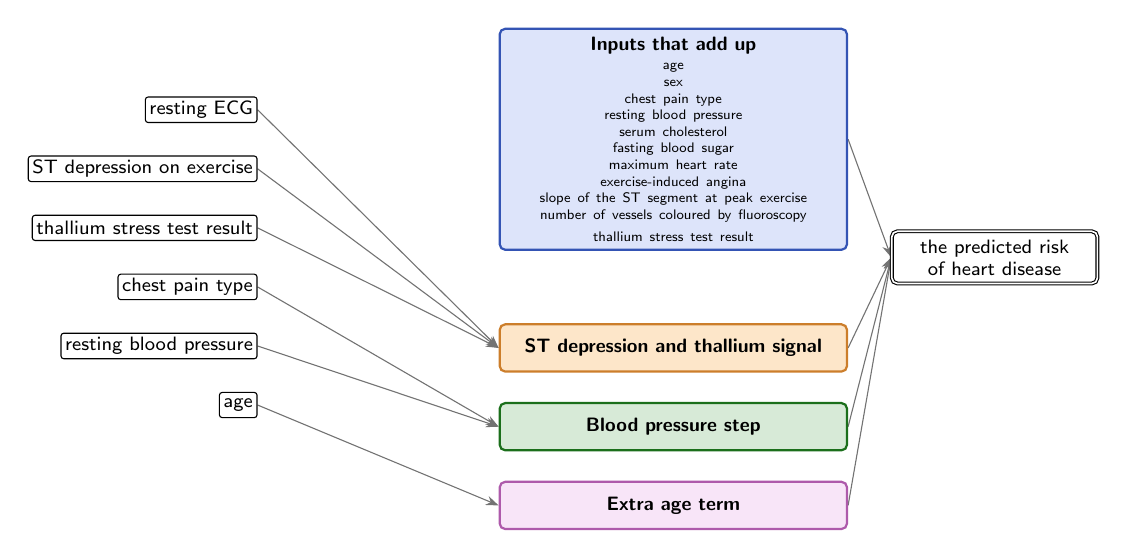
\begin{tikzpicture}[
  font=\sffamily\scriptsize, >={Stealth[length=1.6mm]},
  inp/.style={draw, rounded corners=1pt, fill=white, inner sep=1.5pt, minimum height=3.2mm, anchor=east},
  abox/.style={draw, thick, rounded corners=2pt, align=center, inner sep=3pt, minimum height=6mm, text width=42mm},
  outp/.style={draw, double, rounded corners=2pt, fill=white, align=center, inner sep=3pt, text width=24mm},
  agg/.style={draw=black!55},
]
\node[inp] (i0) at (0,1.875) {resting ECG};
\node[inp] (i1) at (0,1.125) {ST depression on exercise};
\node[inp] (i2) at (0,0.375) {thallium stress test result};
\node[inp] (i3) at (0,-0.375) {chest pain type};
\node[inp] (i4) at (0,-1.125) {resting blood pressure};
\node[inp] (i5) at (0,-1.875) {age};
\node[abox, fill=RoyalBlue!18, draw=RoyalBlue!80!black] (b0) at (5.28,1.5) {\textbf{Inputs that add up}\\[1pt]{\tiny age\\ sex\\ chest pain type\\ resting blood pressure\\ serum cholesterol\\ fasting blood sugar\\ maximum heart rate\\ exercise-induced angina\\ slope of the ST segment at peak exercise\\ number of vessels coloured by fluoroscopy\\ thallium stress test result}};
\node[abox, fill=BurntOrange!18, draw=BurntOrange!80!black] (b1) at (5.28,-1.15) {\textbf{ST depression and thallium signal}};
\node[abox, fill=ForestGreen!18, draw=ForestGreen!80!black] (b2) at (5.28,-2.15) {\textbf{Blood pressure step}};
\node[abox, fill=Orchid!18, draw=Orchid!80!black] (b3) at (5.28,-3.15) {\textbf{Extra age term}};
\node[outp] (out) at (9.36,0) {the predicted risk of heart disease};
\begin{scope}[on background layer]
\draw[->, agg] (b0.east) -- (out.west);
\draw[->, agg, thin] (i0.east) -- (b1.west);
\draw[->, agg, thin] (i1.east) -- (b1.west);
\draw[->, agg, thin] (i2.east) -- (b1.west);
\draw[->, agg] (b1.east) -- (out.west);
\draw[->, agg, thin] (i3.east) -- (b2.west);
\draw[->, agg, thin] (i4.east) -- (b2.west);
\draw[->, agg] (b2.east) -- (out.west);
\draw[->, agg, thin] (i5.east) -- (b3.west);
\draw[->, agg] (b3.east) -- (out.west);
\end{scope}
\end{tikzpicture}}}%
\caption{The whole model: what feeds it, one level down.}
\label{fig:hearts5c1:parts-ann35}
\end{figure}
\begin{figure}[H]\centering
\resizebox{\ifdim\width>\linewidth\linewidth\else\width\fi}{!}{%
\definecolor{netup}{HTML}{D95F02}\definecolor{netdown}{HTML}{1B9E77}\definecolor{netmixed}{HTML}{7F7F7F}%
\begin{tikzpicture}[
  font=\sffamily\scriptsize, >={Stealth[length=1.4mm]},
  inp/.style={draw, circle, fill=white, minimum size=3.2mm, inner sep=0pt},
  hid/.style={draw, circle, fill=white, minimum size=5.2mm, inner sep=0.5pt, font=\sffamily\tiny},
  exitbox/.style={draw, thick, rectangle, fill=white, align=center, text width=17mm, minimum height=5mm, inner sep=1.5pt, font=\sffamily\tiny},
  sumbox/.style={draw, thick, dashed, rectangle, fill=white, align=center, text width=17mm, minimum height=5mm, inner sep=1.5pt, font=\sffamily\tiny},
  outp/.style={draw, thick, regular polygon, regular polygon sides=6, fill=white, minimum size=10mm, inner sep=0pt, font=\sffamily\tiny, align=center},
  stub/.style={draw, dashed, rounded corners=2pt, fill=white, align=center, inner sep=2pt, font=\sffamily\tiny, text width=15mm},
  inlab/.style={font=\sffamily\tiny, align=center, text width=15mm, inner sep=1pt, fill=white, fill opacity=0.8, text opacity=1},
  wpos/.style={draw=NavyBlue}, wneg/.style={draw=BrickRed}, wagg/.style={draw=black!45, line width=1.2pt},
  wmix/.style={draw=Plum},
]
\node[outp] (n0) at (9.32,3.45) {heart disease};
\node[inp, draw=netdown, very thick] (ninxxsexx0) at (2.7,-2.1) {};
\path (ninxxsexx0.south) node[inlab, anchor=north] (labninxxsexx0) {female $\downarrow$};
\node[sumbox] (nxxsumxx) at (5.85,1.9) {sum: Inputs that add up};
\node[inp, draw=netdown, very thick] (ninxxcpx1) at (9.9,0.0) {};
\path (ninxxcpx1.south) node[inlab, anchor=north] (labninxxcpx1) {typical angina $\downarrow$};
\node[inp, draw=netup, very thick] (ninxxcpx4) at (5.4,-1.05) {};
\path (ninxxcpx4.south) node[inlab, anchor=north] (labninxxcpx4) {no chest pain $\uparrow$};
\node[inp, draw=netup, very thick] (ninxxchol) at (1.8,-1.05) {};
\path (ninxxchol.south) node[inlab, anchor=north] (labninxxchol) {cholesterol $\uparrow$};
\node[inp, draw=netup, very thick] (ninxxfbsx0) at (8.1,-2.1) {};
\path (ninxxfbsx0.south) node[inlab, anchor=north] (labninxxfbsx0) {sugar 120 or less $\uparrow$};
\node[inp, draw=netdown, very thick] (ninxxthalach) at (4.5,-2.1) {};
\path (ninxxthalach.south) node[inlab, anchor=north] (labninxxthalach) {max heart rate $\downarrow$};
\node[inp, draw=netdown, very thick] (ninxxexangx0) at (6.3,0.0) {};
\path (ninxxexangx0.south) node[inlab, anchor=north] (labninxxexangx0) {no exercise pain $\downarrow$};
\node[inp, draw=netup, very thick] (ninxxexangx1) at (2.7,0.0) {};
\path (ninxxexangx1.south) node[inlab, anchor=north] (labninxxexangx1) {exercise pain $\uparrow$};
\node[inp, draw=netdown, very thick] (ninxxslopex1) at (9.9,-2.1) {};
\path (ninxxslopex1.south) node[inlab, anchor=north] (labninxxslopex1) {upsloping ST $\downarrow$};
\node[inp, draw=netup, very thick] (ninxxslopex2) at (4.5,0.0) {};
\path (ninxxslopex2.south) node[inlab, anchor=north] (labninxxslopex2) {flat ST $\uparrow$};
\node[inp, draw=netup, very thick] (ninxxslopex3) at (1.8,-3.15) {};
\path (ninxxslopex3.south) node[inlab, anchor=north] (labninxxslopex3) {downsloping ST $\uparrow$};
\node[inp, draw=netup, very thick] (ninxxca) at (10.8,-1.05) {};
\path (ninxxca.south) node[inlab, anchor=north] (labninxxca) {vessels $\uparrow$};
\node[inp, draw=netmixed, very thick] (ninxxthalx3) at (7.2,-1.05) {};
\path (ninxxthalx3.south) node[inlab, anchor=north] (labninxxthalx3) {normal thallium $\updownarrow$};
\node[inp, draw=netup, very thick] (ninxxthalx4) at (9.0,-1.05) {};
\path (ninxxthalx4.south) node[inlab, anchor=north] (labninxxthalx4) {thallium code 4 $\uparrow$};
\node[inp, draw=netdown, very thick] (ninxxthalx6) at (3.6,-1.05) {};
\path (ninxxthalx6.south) node[inlab, anchor=north] (labninxxthalx6) {fixed defect $\downarrow$};
\node[stub] (nfromxxSTxdepressionxandxthalliumxsignal) at (17.74,0.0) {from ST depression and thallium signal};
\node[stub] (nfromxxBloodxpressurexstep) at (14.14,0.0) {from Blood pressure step};
\node[stub] (nfromxxExtraxagexterm) at (15.94,0.0) {from Extra age term};
\node[inp, draw=netup, very thick] (ninxxthalx7) at (8.1,0.0) {};
\path (ninxxthalx7.south) node[inlab, anchor=north] (labninxxthalx7) {reversible defect $\uparrow$};
\node[inp, draw=netdown, very thick] (ninxxcpx3) at (6.3,-2.1) {};
\path (ninxxcpx3.south) node[inlab, anchor=north] (labninxxcpx3) {non-anginal pain $\downarrow$};
\node[inp, draw=netup, very thick] (ninxxtrestbps) at (0.9,-2.1) {};
\path (ninxxtrestbps.south) node[inlab, anchor=north] (labninxxtrestbps) {blood pressure $\uparrow$};
\node[inp, draw=netup, very thick] (ninxxage) at (0.9,0.0) {};
\path (ninxxage.south) node[inlab, anchor=north] (labninxxage) {age $\uparrow$};
\begin{scope}[on background layer]
\node[fit=(nxxsumxx) , inner sep=8pt, rounded corners=5pt, fill=RoyalBlue!10, draw=RoyalBlue!45] (clu0) {};
\draw[->, wneg, line width=0.63pt] (ninxxsexx0) -- (nxxsumxx);
\draw[->, wneg, line width=0.42pt] (ninxxcpx1) -- (nxxsumxx);
\draw[->, wpos, line width=0.38pt] (ninxxcpx4) -- (nxxsumxx);
\draw[->, wpos, line width=0.44pt] (ninxxchol) -- (nxxsumxx);
\draw[->, wpos, line width=0.35pt] (ninxxfbsx0) -- (nxxsumxx);
\draw[->, wneg, line width=0.32pt] (ninxxthalach) -- (nxxsumxx);
\draw[->, wpos, line width=0.30pt] (ninxxexangx0) -- (nxxsumxx);
\draw[->, wpos, line width=0.40pt] (ninxxexangx1) -- (nxxsumxx);
\draw[->, wneg, line width=0.55pt] (ninxxslopex1) -- (nxxsumxx);
\draw[->, wpos, line width=0.30pt] (ninxxslopex2) -- (nxxsumxx);
\draw[->, wneg, line width=0.38pt] (ninxxslopex3) -- (nxxsumxx);
\draw[->, wpos, line width=0.77pt] (ninxxca) -- (nxxsumxx);
\draw[->, wneg, line width=0.39pt] (ninxxthalx3) -- (nxxsumxx);
\draw[->, wpos, line width=0.31pt] (ninxxthalx4) -- (nxxsumxx);
\draw[->, wneg, line width=0.38pt] (ninxxthalx6) -- (nxxsumxx);
\draw[->, wpos, line width=0.30pt] (nfromxxSTxdepressionxandxthalliumxsignal) -- (n0);
\draw[->, wpos, line width=0.31pt] (nfromxxBloodxpressurexstep) -- (n0);
\draw[->, wpos, line width=0.30pt] (nfromxxExtraxagexterm) -- (n0);
\draw[->, wneg, line width=0.28pt] (ninxxthalx7) -- (nxxsumxx);
\draw[->, wneg, line width=0.40pt] (ninxxcpx3) -- (nxxsumxx);
\draw[->, wpos, line width=0.42pt] (ninxxtrestbps) -- (nxxsumxx);
\draw[->, wpos, line width=0.29pt] (ninxxage) -- (nxxsumxx);
\draw[->, wagg] (nxxsumxx) -- (n0);
\end{scope}
\node[font=\sffamily\scriptsize\bfseries, text=RoyalBlue!55!black, anchor=south west, inner sep=1pt, fill=white, fill opacity=0.85, text opacity=1] at (clu0.north west) {Inputs that add up};
\end{tikzpicture}}%
\caption{The whole model: its units and every connection into them. Blue: positive weight (raises the score); red: negative weight (lowers it); thicker: larger weight. Orange outline and up arrow: raises the final prediction; teal and down arrow: lowers it; grey and double arrow: depends.}
\label{fig:hearts5c1:units-ann35}
\end{figure}
\paragraph{Hypothesis.} The model adds up its inputs into one score: the vessels coloured (each extra vessel adding about the same), the ST segment, sex and chest pain type each move the predicted risk on their own, and a chain of three parts adds to that sum: a signal from ST depression and the thallium scan, a blood pressure step that reads it, and an extra age term after that.\,{\scriptsize\textcolor{NavyBlue}{[C32, C01, C04, C12, C10]}}
\paragraph{Evidence.} It is made up of the inputs that feed the score directly and three parts, the ST depression and thallium signal, the blood pressure step and the extra age term (each explained below); the first part feeds the second and the second feeds the third, and the score is their sum, which was checked on all 242 training patients.\,{\scriptsize\textcolor{NavyBlue}{[C32]}} ST depression on exercise and the resting ECG do not feed the score directly, so they act only through these parts.\,{\scriptsize\textcolor{NavyBlue}{[C32, C33]}} Changing one input at a time across the whole model, more ST depression raises a typical patient's predicted risk in an uneven way, from about 22\% at 0 mm to about 48\% at 2.8 mm, and a reversible defect on the thallium scan takes it to about 47\%, against about 35\% through the sum alone.\,{\scriptsize\textcolor{NavyBlue}{[C05, C06, C15]}} Across the whole model, higher resting blood pressure raises it in an uneven way, from about 14\% at 110 mm Hg to about 35\% at 155 mm Hg, and older age raises it in an uneven way, from about 18\% at 42 to about 26\% at 66 years.\,{\scriptsize\textcolor{NavyBlue}{[C09, C23]}} Across the whole model, a fixed defect on the thallium scan lowers it to about 11\% (the model has little data on this, n = 15), and a resting ECG other than normal barely changes it for a typical patient.\,{\scriptsize\textcolor{NavyBlue}{[C19, C26]}}
\par\noindent{\small Evidence plots: Figure~\ref{fig:hearts5c1:plot-ann35-0}.\par}
\begin{figure}[H]\centering
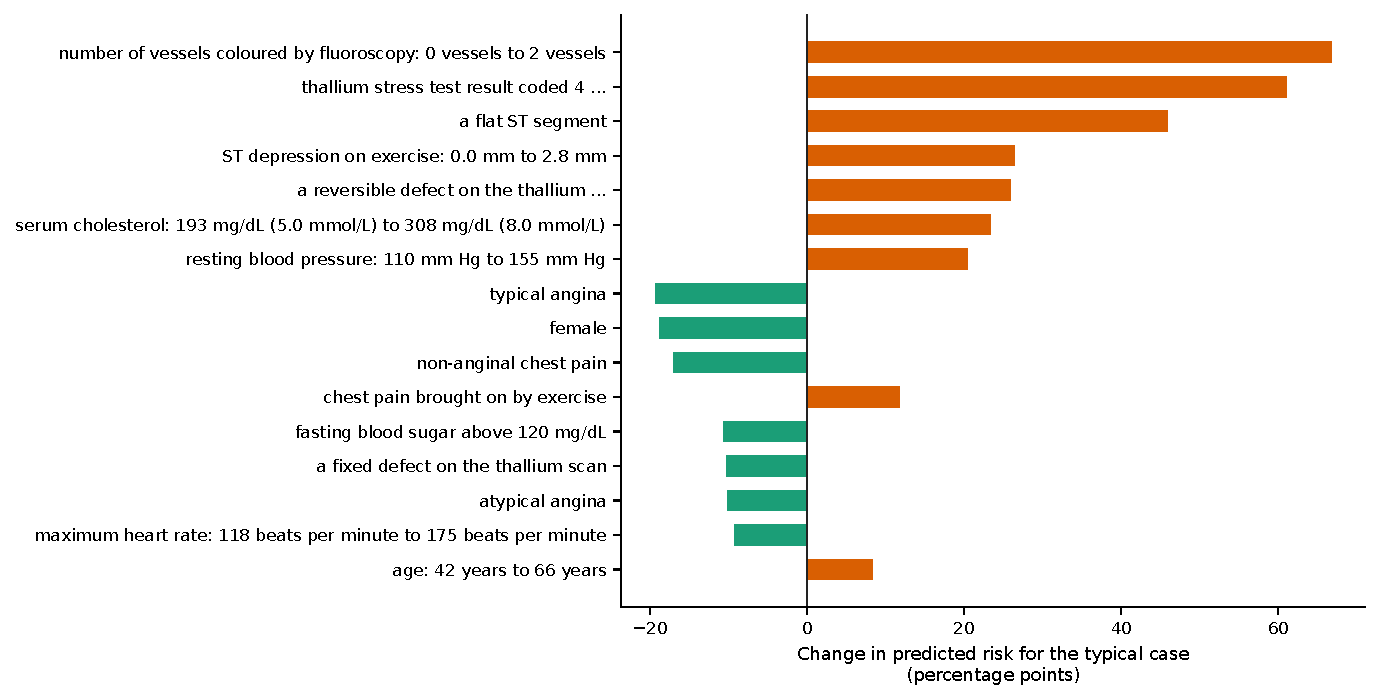
\includegraphics[width=\linewidth,height=0.88\textheight,keepaspectratio]{figures/heart-s5-c1/ann_35-effects.pdf}
\caption{The whole model: Each input's change in the predicted value for the typical case across the whole model, largest first (orange: raises it, teal: lowers it).}
\label{fig:hearts5c1:plot-ann35-0}
\end{figure}
\par\smallskip\noindent{\small \textbf{Dive deeper:} ST depression and thallium signal (\ref{rd:ann32}); Blood pressure step (\ref{rd:ann33}); Extra age term (\ref{rd:ann34}). Technical detail: \ref{tech:ann35}.\par}
\subsubsection{ST depression and thallium signal}\label{rd:ann32}
\noindent{\footnotesize Part of: The whole model (\ref{rd:ann35}).\par}
\noindent{\small Figure~\ref{fig:hearts5c1:parts-ann32} shows what feeds this part; Figure~\ref{fig:hearts5c1:units-ann32} its units and every connection into them (dashed boxes: connections from or to other parts, drawn in their own sections).\par}
\begin{figure}[H]\centering
\resizebox{!}{\ifdim\height>0.5\textheight 0.5\textheight\else\height\fi}{%
\resizebox{\ifdim\width>\linewidth\linewidth\else\width\fi}{!}{%
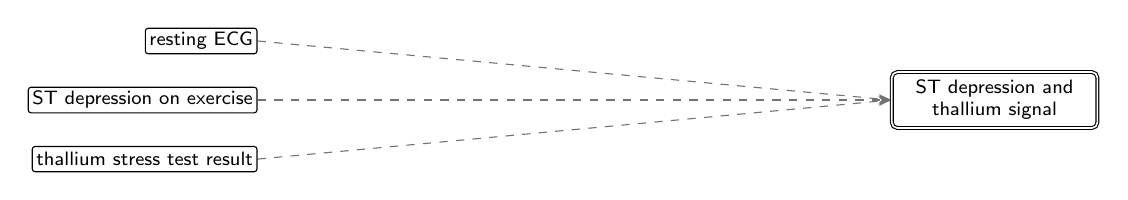
\begin{tikzpicture}[
  font=\sffamily\scriptsize, >={Stealth[length=1.6mm]},
  inp/.style={draw, rounded corners=1pt, fill=white, inner sep=1.5pt, minimum height=3.2mm, anchor=east},
  abox/.style={draw, thick, rounded corners=2pt, align=center, inner sep=3pt, minimum height=6mm, text width=42mm},
  outp/.style={draw, double, rounded corners=2pt, fill=white, align=center, inner sep=3pt, text width=24mm},
  agg/.style={draw=black!55},
]
\node[inp] (i0) at (0,0.75) {resting ECG};
\node[inp] (i1) at (0,-0.0) {ST depression on exercise};
\node[inp] (i2) at (0,-0.75) {thallium stress test result};
\node[outp] (out) at (9.36,0) {ST depression and thallium signal};
\begin{scope}[on background layer]
\draw[->, agg, thin, dashed] (i0.east) -- (out.west);
\draw[->, agg, thin, dashed] (i1.east) -- (out.west);
\draw[->, agg, thin, dashed] (i2.east) -- (out.west);
\end{scope}
\end{tikzpicture}}}%
\caption{ST depression and thallium signal: what feeds it, one level down.}
\label{fig:hearts5c1:parts-ann32}
\end{figure}
\begin{figure}[H]\centering
\resizebox{\ifdim\width>\linewidth\linewidth\else\width\fi}{!}{%
\definecolor{netup}{HTML}{D95F02}\definecolor{netdown}{HTML}{1B9E77}\definecolor{netmixed}{HTML}{7F7F7F}%
\begin{tikzpicture}[
  font=\sffamily\scriptsize, >={Stealth[length=1.4mm]},
  inp/.style={draw, circle, fill=white, minimum size=3.2mm, inner sep=0pt},
  hid/.style={draw, circle, fill=white, minimum size=5.2mm, inner sep=0.5pt, font=\sffamily\tiny},
  exitbox/.style={draw, thick, rectangle, fill=white, align=center, text width=17mm, minimum height=5mm, inner sep=1.5pt, font=\sffamily\tiny},
  sumbox/.style={draw, thick, dashed, rectangle, fill=white, align=center, text width=17mm, minimum height=5mm, inner sep=1.5pt, font=\sffamily\tiny},
  outp/.style={draw, thick, regular polygon, regular polygon sides=6, fill=white, minimum size=10mm, inner sep=0pt, font=\sffamily\tiny, align=center},
  stub/.style={draw, dashed, rounded corners=2pt, fill=white, align=center, inner sep=2pt, font=\sffamily\tiny, text width=15mm},
  inlab/.style={font=\sffamily\tiny, align=center, text width=15mm, inner sep=1pt, fill=white, fill opacity=0.8, text opacity=1},
  wpos/.style={draw=NavyBlue}, wneg/.style={draw=BrickRed}, wagg/.style={draw=black!45, line width=1.2pt},
  wmix/.style={draw=Plum},
]
\node[exitbox] (n204) at (3.3,1.9) {ST depression and thallium signal $\updownarrow$};
\node[inp, draw=netup, very thick] (ninxxrestecgx0) at (3.3,0.0) {};
\path (ninxxrestecgx0.south) node[inlab, anchor=north] (labninxxrestecgx0) {normal ECG $\uparrow$};
\node[inp, draw=netup, very thick] (ninxxoldpeak) at (1.5,0.0) {};
\path (ninxxoldpeak.south) node[inlab, anchor=north] (labninxxoldpeak) {ST depression $\uparrow$};
\node[inp, draw=netup, very thick] (ninxxthalx7) at (5.1,0.0) {};
\path (ninxxthalx7.south) node[inlab, anchor=north] (labninxxthalx7) {reversible defect $\uparrow$};
\node[stub] (ntoxxthexmodelxoutput) at (1.8,3.45) {to the model output};
\node[stub] (ntoxxBloodxpressurexstep) at (4.8,3.45) {to Blood pressure step};
\begin{scope}[on background layer]
\node[fit=(n204) , inner sep=8pt, rounded corners=5pt, fill=BurntOrange!10, draw=BurntOrange!45] (clu0) {};
\draw[->, wpos, line width=0.55pt] (ninxxrestecgx0) -- (n204);
\draw[->, wpos, line width=1.16pt] (ninxxoldpeak) -- (n204);
\draw[->, wpos, line width=0.65pt] (ninxxthalx7) -- (n204);
\draw[->, wpos, line width=0.30pt] (n204) -- (ntoxxthexmodelxoutput);
\draw[->, wpos, line width=0.63pt] (n204) -- (ntoxxBloodxpressurexstep);
\end{scope}
\node[font=\sffamily\scriptsize\bfseries, text=BurntOrange!55!black, anchor=south west, inner sep=1pt, fill=white, fill opacity=0.85, text opacity=1] at (clu0.north west) {ST depression and thallium signal};
\end{tikzpicture}}%
\caption{ST depression and thallium signal: its units and every connection into them. Blue: positive weight (raises the score); red: negative weight (lowers it); thicker: larger weight. Orange outline and up arrow: raises the final prediction; teal and down arrow: lowers it; grey and double arrow: depends.}
\label{fig:hearts5c1:units-ann32}
\end{figure}
\paragraph{Hypothesis.} This part raises the predicted risk with ST depression on exercise once it rises above about 0.9 mm, in an uneven way, and more so with a reversible defect on the thallium scan or a normal resting ECG.\,{\scriptsize\textcolor{NavyBlue}{[C33, C39, C36, C37]}}
\paragraph{Evidence.} It acts on 116 of 242 training patients, 77 of whom had heart disease; for the typical patient it acts on, the predicted risk is about 89\% without it and about 96\% with it.\,{\scriptsize\textcolor{NavyBlue}{[C40]}} Through it, more ST depression adds to the risk only once it rises above about 0.9 mm, rising in an uneven way: for a typical patient from about 22\% at 0 mm to about 48\% at 2.8 mm.\,{\scriptsize\textcolor{NavyBlue}{[C33, C39]}} ST depression counts more with a reversible defect on the thallium scan (from about 36\% to about 80\%, against about 22\% to about 48\% otherwise) and with a normal resting ECG (from about 22\% to about 48\%, against about 22\% to about 34\% otherwise), in an uneven way.\,{\scriptsize\textcolor{NavyBlue}{[C36, C37]}} Through it, a reversible defect on the thallium scan raises a typical patient's risk from about 22\% to about 32\%, and more with a normal resting ECG (to about 47\%, against about 36\% otherwise).\,{\scriptsize\textcolor{NavyBlue}{[C34, C38]}} Its formula reproduces the part exactly on all 242 training patients.\,{\scriptsize\textcolor{NavyBlue}{[C41]}}
\par\noindent{\small Evidence plots: Figure~\ref{fig:hearts5c1:plot-ann32-0}, Figure~\ref{fig:hearts5c1:plot-ann32-1}, Figure~\ref{fig:hearts5c1:plot-ann32-2}, Figure~\ref{fig:hearts5c1:plot-ann32-3}, Figure~\ref{fig:hearts5c1:plot-ann32-4}.\par}
\par\noindent{\small Figure~\ref{fig:hearts5c1:plot-ann32-3} shows this part's own output, unit h1: it switches on at about 0.9273 mm of ST depression on exercise, and is zero below.\par}
\begin{figure}[H]\centering
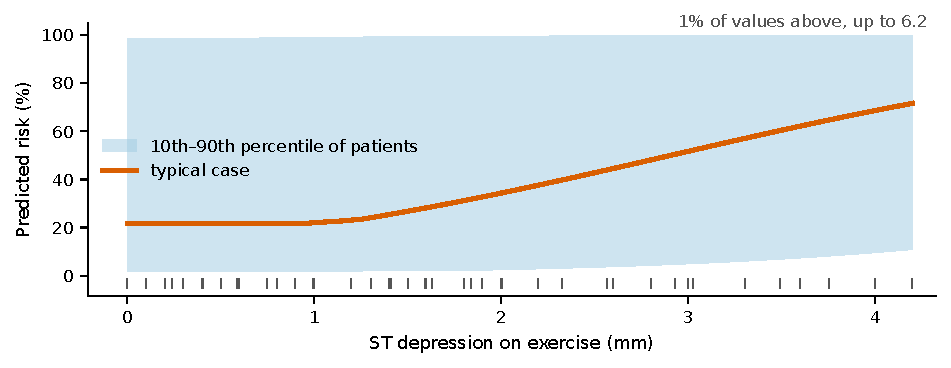
\includegraphics[width=\linewidth,height=0.88\textheight,keepaspectratio]{figures/heart-s5-c1/ann_32-response.pdf}
\caption{ST depression and thallium signal: Response curves through this part: the typical case (bold), the 10th to 90th percentile of individual patients (band), the fold or step point (dashed) with its spread across them (grey), and the observed values (ticks).}
\label{fig:hearts5c1:plot-ann32-0}
\end{figure}
\begin{figure}[H]\centering
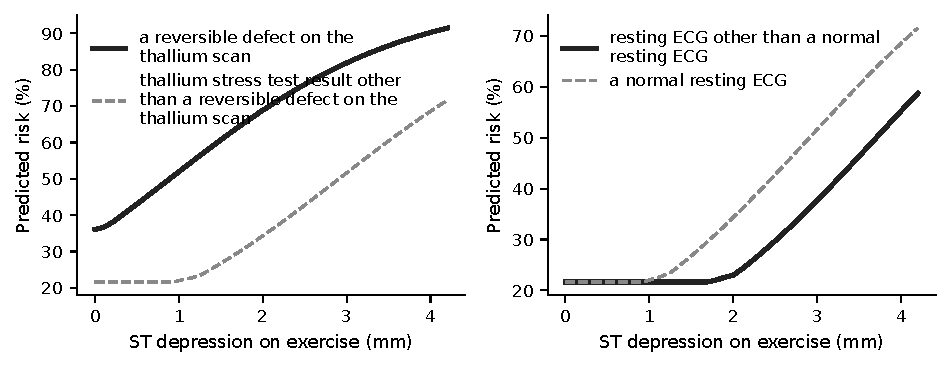
\includegraphics[width=\linewidth,height=0.88\textheight,keepaspectratio]{figures/heart-s5-c1/ann_32-interaction.pdf}
\caption{ST depression and thallium signal: How the effect differs between groups: one curve per group, for the typical case of each group.}
\label{fig:hearts5c1:plot-ann32-1}
\end{figure}
\begin{figure}[H]\centering
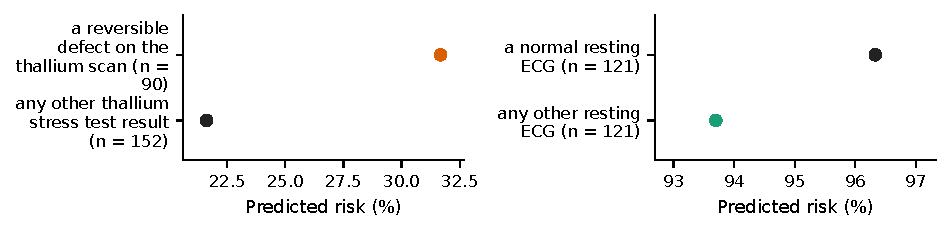
\includegraphics[width=\linewidth,height=0.88\textheight,keepaspectratio]{figures/heart-s5-c1/ann_32-categories-small.pdf}
\caption{ST depression and thallium signal: The predicted value for the typical case at each level, through this part (n = training patients; grey: fewer than 20).}
\label{fig:hearts5c1:plot-ann32-2}
\end{figure}
\begin{figure}[H]\centering
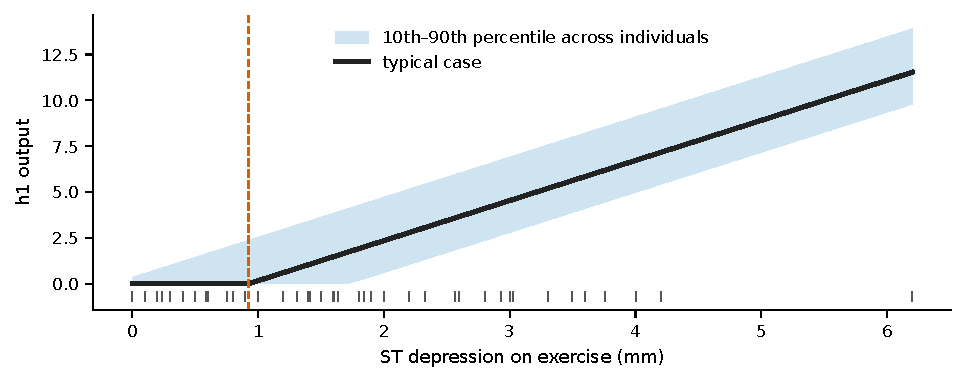
\includegraphics[width=\linewidth,height=0.88\textheight,keepaspectratio]{figures/heart-s5-c1/ann_32-partial-204.pdf}
\caption{ST depression and thallium signal: This part's own output, unit h1 (the output of 'ST depression and thallium signal'), on its own scale (its activation), with every other input at the typical case; it is active for 116 of 242. Bold: the typical case; band: 10th to 90th percentile across individuals; dashed: where it switches on; ticks: the data.}
\label{fig:hearts5c1:plot-ann32-3}
\end{figure}
\begin{figure}[H]\centering
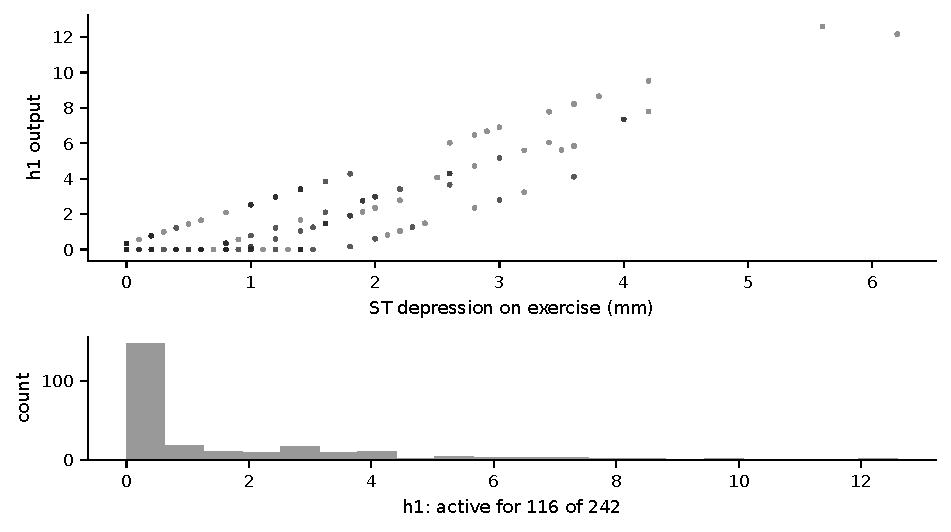
\includegraphics[width=\linewidth,height=0.88\textheight,keepaspectratio]{figures/heart-s5-c1/ann_32-units.pdf}
\caption{ST depression and thallium signal: This part's hidden units: each unit's output against its main numeric input (top) and how often it is active (bottom).}
\label{fig:hearts5c1:plot-ann32-4}
\end{figure}
\par\smallskip\noindent{\small Technical detail: \ref{tech:ann32}.\par}
\subsubsection{Blood pressure step}\label{rd:ann33}
\noindent{\footnotesize Part of: The whole model (\ref{rd:ann35}).\par}
\noindent{\small Figure~\ref{fig:hearts5c1:parts-ann33} shows what feeds this part; Figure~\ref{fig:hearts5c1:units-ann33} its units and every connection into them (dashed boxes: connections from or to other parts, drawn in their own sections).\par}
\begin{figure}[H]\centering
\resizebox{!}{\ifdim\height>0.5\textheight 0.5\textheight\else\height\fi}{%
\resizebox{\ifdim\width>\linewidth\linewidth\else\width\fi}{!}{%
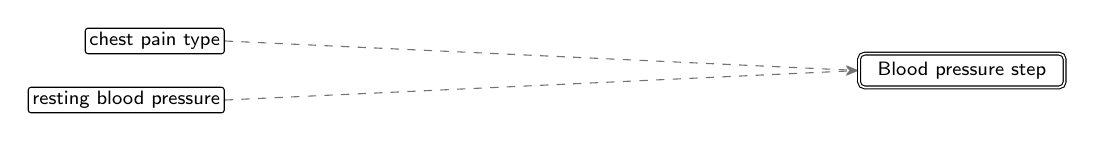
\begin{tikzpicture}[
  font=\sffamily\scriptsize, >={Stealth[length=1.6mm]},
  inp/.style={draw, rounded corners=1pt, fill=white, inner sep=1.5pt, minimum height=3.2mm, anchor=east},
  abox/.style={draw, thick, rounded corners=2pt, align=center, inner sep=3pt, minimum height=6mm, text width=42mm},
  outp/.style={draw, double, rounded corners=2pt, fill=white, align=center, inner sep=3pt, text width=24mm},
  agg/.style={draw=black!55},
]
\node[inp] (i0) at (0,0.375) {chest pain type};
\node[inp] (i1) at (0,-0.375) {resting blood pressure};
\node[outp] (out) at (9.36,0) {Blood pressure step};
\begin{scope}[on background layer]
\draw[->, agg, thin, dashed] (i0.east) -- (out.west);
\draw[->, agg, thin, dashed] (i1.east) -- (out.west);
\end{scope}
\end{tikzpicture}}}%
\caption{Blood pressure step: what feeds it, one level down.}
\label{fig:hearts5c1:parts-ann33}
\end{figure}
\begin{figure}[H]\centering
\resizebox{\ifdim\width>\linewidth\linewidth\else\width\fi}{!}{%
\definecolor{netup}{HTML}{D95F02}\definecolor{netdown}{HTML}{1B9E77}\definecolor{netmixed}{HTML}{7F7F7F}%
\begin{tikzpicture}[
  font=\sffamily\scriptsize, >={Stealth[length=1.4mm]},
  inp/.style={draw, circle, fill=white, minimum size=3.2mm, inner sep=0pt},
  hid/.style={draw, circle, fill=white, minimum size=5.2mm, inner sep=0.5pt, font=\sffamily\tiny},
  exitbox/.style={draw, thick, rectangle, fill=white, align=center, text width=17mm, minimum height=5mm, inner sep=1.5pt, font=\sffamily\tiny},
  sumbox/.style={draw, thick, dashed, rectangle, fill=white, align=center, text width=17mm, minimum height=5mm, inner sep=1.5pt, font=\sffamily\tiny},
  outp/.style={draw, thick, regular polygon, regular polygon sides=6, fill=white, minimum size=10mm, inner sep=0pt, font=\sffamily\tiny, align=center},
  stub/.style={draw, dashed, rounded corners=2pt, fill=white, align=center, inner sep=2pt, font=\sffamily\tiny, text width=15mm},
  inlab/.style={font=\sffamily\tiny, align=center, text width=15mm, inner sep=1pt, fill=white, fill opacity=0.8, text opacity=1},
  wpos/.style={draw=NavyBlue}, wneg/.style={draw=BrickRed}, wagg/.style={draw=black!45, line width=1.2pt},
  wmix/.style={draw=Plum},
]
\node[exitbox] (n290) at (3.6,3.25) {Blood pressure step $\updownarrow$};
\node[hid] (nidentityx290) at (3.6,1.9) {h4};
\node[inp, draw=netup, very thick] (ninxxcpx2) at (0.9,0.0) {};
\path (ninxxcpx2.south) node[inlab, anchor=north] (labninxxcpx2) {atypical angina $\uparrow$};
\node[inp, draw=netup, very thick] (ninxxcpx3) at (6.3,0.0) {};
\path (ninxxcpx3.south) node[inlab, anchor=north] (labninxxcpx3) {non-anginal pain $\uparrow$};
\node[inp, draw=netup, very thick] (ninxxtrestbps) at (2.7,0.0) {};
\path (ninxxtrestbps.south) node[inlab, anchor=north] (labninxxtrestbps) {blood pressure $\uparrow$};
\node[stub] (nfromxxSTxdepressionxandxthalliumxsignal) at (4.5,0.0) {from ST depression and thallium signal};
\node[stub] (ntoxxthexmodelxoutput) at (2.1,4.8) {to the model output};
\node[stub] (ntoxxExtraxagexterm) at (5.1,4.8) {to Extra age term};
\begin{scope}[on background layer]
\node[fit=(n290) (nidentityx290) , inner sep=8pt, rounded corners=5pt, fill=ForestGreen!10, draw=ForestGreen!45] (clu0) {};
\draw[->, wpos, line width=0.31pt] (ninxxcpx2) -- (n290);
\draw[->, wpos, line width=0.26pt] (ninxxcpx3) -- (n290);
\draw[->, wneg, line width=0.54pt] (ninxxtrestbps) -- (n290);
\draw[->, wpos, line width=0.63pt] (nfromxxSTxdepressionxandxthalliumxsignal) -- (nidentityx290);
\draw[->, wpos, line width=0.60pt] (nidentityx290) -- (n290);
\draw[->, wpos, line width=0.31pt] (n290) -- (ntoxxthexmodelxoutput);
\draw[->, wneg, line width=0.81pt] (n290) -- (ntoxxExtraxagexterm);
\end{scope}
\node[font=\sffamily\scriptsize\bfseries, text=ForestGreen!55!black, anchor=south west, inner sep=1pt, fill=white, fill opacity=0.85, text opacity=1] at (clu0.north west) {Blood pressure step};
\end{tikzpicture}}%
\caption{Blood pressure step: its units and every connection into them. Blue: positive weight (raises the score); red: negative weight (lowers it); thicker: larger weight. Orange outline and up arrow: raises the final prediction; teal and down arrow: lowers it; grey and double arrow: depends.}
\label{fig:hearts5c1:units-ann33}
\end{figure}
\paragraph{Hypothesis.} This part reads the ST depression and thallium signal together with resting blood pressure and chest pain type, and barely changes the predictions for the typical patient it acts on.\,{\scriptsize\textcolor{NavyBlue}{[C42, C44]}}
\paragraph{Evidence.} For the typical patient it acts on, atypical angina raises the predicted risk through it from about 69\% to about 70\%, and non-anginal chest pain leaves it at about 69\%.\,{\scriptsize\textcolor{NavyBlue}{[C42, C44]}} Its formula reproduces the part exactly on all 242 training patients.\,{\scriptsize\textcolor{NavyBlue}{[C48]}}
\par\noindent{\small Evidence plots: Figure~\ref{fig:hearts5c1:plot-ann33-0}, Figure~\ref{fig:hearts5c1:plot-ann33-1}, Figure~\ref{fig:hearts5c1:plot-ann33-2}.\par}
\par\noindent{\small Figure~\ref{fig:hearts5c1:plot-ann33-1} shows this part's own output, unit h2: over its two main inputs, with the line where it switches on.\par}
\begin{figure}[H]\centering
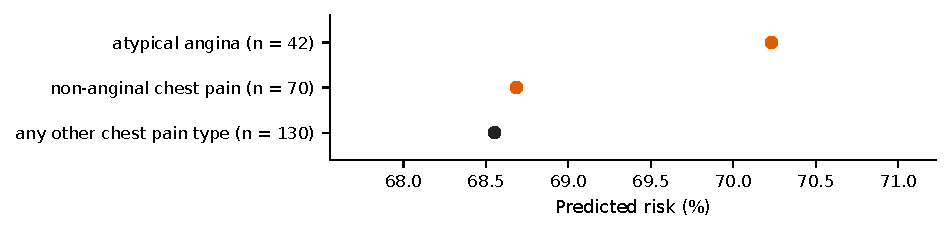
\includegraphics[width=\linewidth,height=0.88\textheight,keepaspectratio]{figures/heart-s5-c1/ann_33-categories-small.pdf}
\caption{Blood pressure step: The predicted value for the typical case at each level, through this part (n = training patients; grey: fewer than 20).}
\label{fig:hearts5c1:plot-ann33-0}
\end{figure}
\begin{figure}[H]\centering
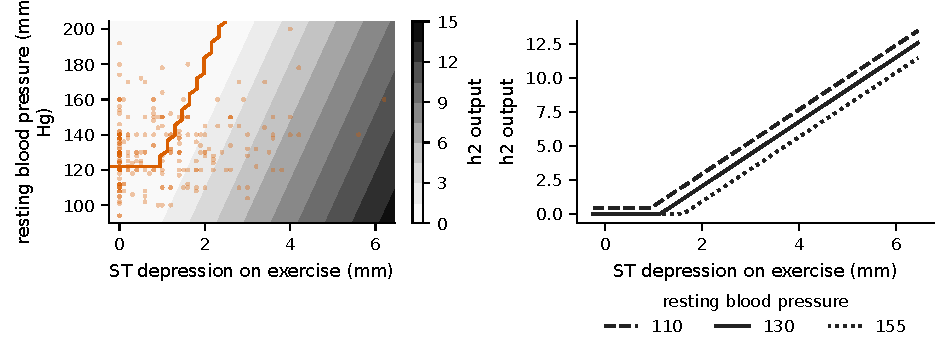
\includegraphics[width=\linewidth,height=0.88\textheight,keepaspectratio]{figures/heart-s5-c1/ann_33-partial-290.pdf}
\caption{Blood pressure step: This part's own output, unit h2 (the output of 'Blood pressure step'), on its own scale (its activation), with every other input at the typical case; it is active for 140 of 242. Left: its output over its two main inputs (orange line: where it switches on; dots: the data); right: slices at three values of the second input.}
\label{fig:hearts5c1:plot-ann33-1}
\end{figure}
\begin{figure}[H]\centering
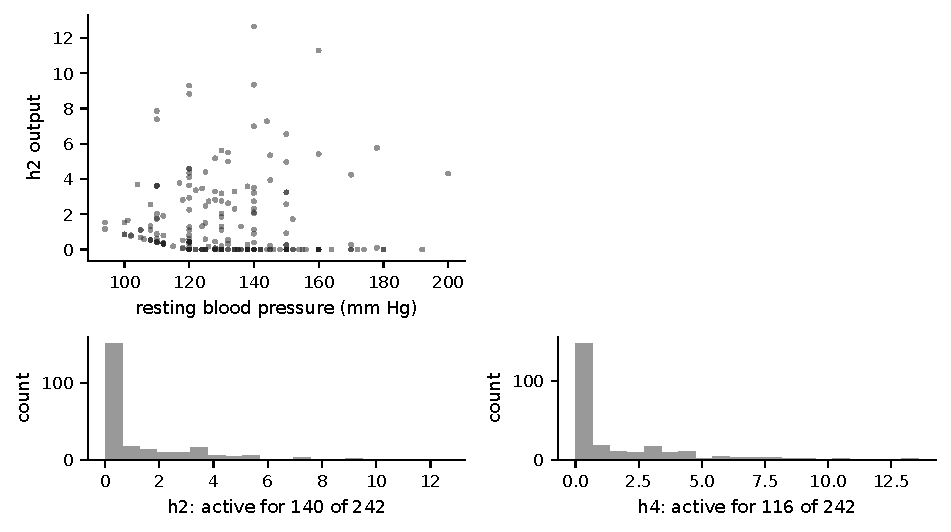
\includegraphics[width=\linewidth,height=0.88\textheight,keepaspectratio]{figures/heart-s5-c1/ann_33-units.pdf}
\caption{Blood pressure step: This part's hidden units: each unit's output against its main numeric input (top) and how often it is active (bottom).}
\label{fig:hearts5c1:plot-ann33-2}
\end{figure}
\par\smallskip\noindent{\small Technical detail: \ref{tech:ann33}.\par}
\subsubsection{Extra age term}\label{rd:ann34}
\noindent{\footnotesize Part of: The whole model (\ref{rd:ann35}).\par}
\noindent{\small Figure~\ref{fig:hearts5c1:parts-ann34} shows what feeds this part; Figure~\ref{fig:hearts5c1:units-ann34} its units and every connection into them (dashed boxes: connections from or to other parts, drawn in their own sections).\par}
\begin{figure}[H]\centering
\resizebox{!}{\ifdim\height>0.5\textheight 0.5\textheight\else\height\fi}{%
\resizebox{\ifdim\width>\linewidth\linewidth\else\width\fi}{!}{%
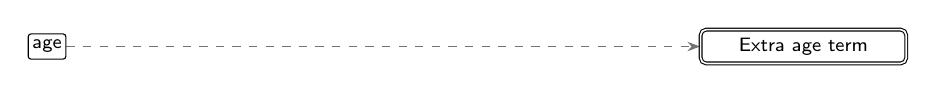
\begin{tikzpicture}[
  font=\sffamily\scriptsize, >={Stealth[length=1.6mm]},
  inp/.style={draw, rounded corners=1pt, fill=white, inner sep=1.5pt, minimum height=3.2mm, anchor=east},
  abox/.style={draw, thick, rounded corners=2pt, align=center, inner sep=3pt, minimum height=6mm, text width=42mm},
  outp/.style={draw, double, rounded corners=2pt, fill=white, align=center, inner sep=3pt, text width=24mm},
  agg/.style={draw=black!55},
]
\node[inp] (i0) at (0,-0.0) {age};
\node[outp] (out) at (9.36,0) {Extra age term};
\begin{scope}[on background layer]
\draw[->, agg, thin, dashed] (i0.east) -- (out.west);
\end{scope}
\end{tikzpicture}}}%
\caption{Extra age term: what feeds it, one level down.}
\label{fig:hearts5c1:parts-ann34}
\end{figure}
\begin{figure}[H]\centering
\resizebox{\ifdim\width>\linewidth\linewidth\else\width\fi}{!}{%
\definecolor{netup}{HTML}{D95F02}\definecolor{netdown}{HTML}{1B9E77}\definecolor{netmixed}{HTML}{7F7F7F}%
\begin{tikzpicture}[
  font=\sffamily\scriptsize, >={Stealth[length=1.4mm]},
  inp/.style={draw, circle, fill=white, minimum size=3.2mm, inner sep=0pt},
  hid/.style={draw, circle, fill=white, minimum size=5.2mm, inner sep=0.5pt, font=\sffamily\tiny},
  exitbox/.style={draw, thick, rectangle, fill=white, align=center, text width=17mm, minimum height=5mm, inner sep=1.5pt, font=\sffamily\tiny},
  sumbox/.style={draw, thick, dashed, rectangle, fill=white, align=center, text width=17mm, minimum height=5mm, inner sep=1.5pt, font=\sffamily\tiny},
  outp/.style={draw, thick, regular polygon, regular polygon sides=6, fill=white, minimum size=10mm, inner sep=0pt, font=\sffamily\tiny, align=center},
  stub/.style={draw, dashed, rounded corners=2pt, fill=white, align=center, inner sep=2pt, font=\sffamily\tiny, text width=15mm},
  inlab/.style={font=\sffamily\tiny, align=center, text width=15mm, inner sep=1pt, fill=white, fill opacity=0.8, text opacity=1},
  wpos/.style={draw=NavyBlue}, wneg/.style={draw=BrickRed}, wagg/.style={draw=black!45, line width=1.2pt},
  wmix/.style={draw=Plum},
]
\node[exitbox] (n1987) at (1.8,3.25) {Extra age term $\uparrow$};
\node[hid] (nidentityx1987) at (1.8,1.9) {h5};
\node[inp, draw=netup, very thick] (ninxxage) at (0.9,0.0) {};
\path (ninxxage.south) node[inlab, anchor=north] (labninxxage) {age $\uparrow$};
\node[stub] (nfromxxBloodxpressurexstep) at (2.7,0.0) {from Blood pressure step};
\node[stub] (ntoxxthexmodelxoutput) at (1.8,4.8) {to the model output};
\begin{scope}[on background layer]
\node[fit=(n1987) (nidentityx1987) , inner sep=8pt, rounded corners=5pt, fill=Orchid!10, draw=Orchid!45] (clu0) {};
\draw[->, wpos, line width=0.56pt] (ninxxage) -- (n1987);
\draw[->, wneg, line width=0.81pt] (nfromxxBloodxpressurexstep) -- (nidentityx1987);
\draw[->, wpos, line width=0.60pt] (nidentityx1987) -- (n1987);
\draw[->, wpos, line width=0.30pt] (n1987) -- (ntoxxthexmodelxoutput);
\end{scope}
\node[font=\sffamily\scriptsize\bfseries, text=Orchid!55!black, anchor=south west, inner sep=1pt, fill=white, fill opacity=0.85, text opacity=1] at (clu0.north west) {Extra age term};
\end{tikzpicture}}%
\caption{Extra age term: its units and every connection into them. Blue: positive weight (raises the score); red: negative weight (lowers it); thicker: larger weight. Orange outline and up arrow: raises the final prediction; teal and down arrow: lowers it; grey and double arrow: depends.}
\label{fig:hearts5c1:units-ann34}
\end{figure}
\paragraph{Hypothesis.} This part adds a little to the predicted risk for older patients: nothing until about 53 years, then steadily.\,{\scriptsize\textcolor{NavyBlue}{[C49, C50]}}
\paragraph{Evidence.} It acts on 85 of 242 training patients, 37 of whom had heart disease; for the typical patient it acts on, the predicted risk is about 28\% without it and about 30\% with it.\,{\scriptsize\textcolor{NavyBlue}{[C51]}} Through it, age adds nothing until about 53 years (between 53 and 66 years for different patients), then raises the risk steadily, for a typical patient from about 21\% at 42 to about 24\% at 66 years.\,{\scriptsize\textcolor{NavyBlue}{[C49, C50]}} Its formula reproduces the part exactly on all 242 training patients.\,{\scriptsize\textcolor{NavyBlue}{[C52]}}
\par\noindent{\small Evidence plots: Figure~\ref{fig:hearts5c1:plot-ann34-0}, Figure~\ref{fig:hearts5c1:plot-ann34-1}, Figure~\ref{fig:hearts5c1:plot-ann34-2}.\par}
\par\noindent{\small Figure~\ref{fig:hearts5c1:plot-ann34-1} shows this part's own output, unit h3: over its two main inputs, with the line where it switches on.\par}
\begin{figure}[H]\centering
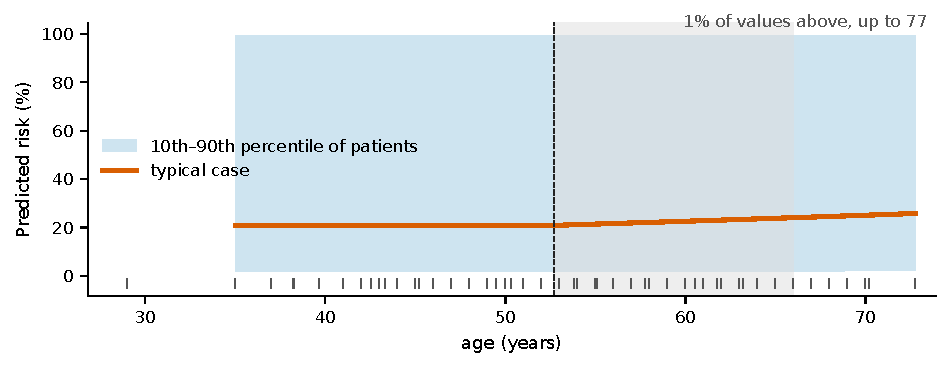
\includegraphics[width=\linewidth,height=0.88\textheight,keepaspectratio]{figures/heart-s5-c1/ann_34-response.pdf}
\caption{Extra age term: Response curves through this part: the typical case (bold), the 10th to 90th percentile of individual patients (band), the fold or step point (dashed) with its spread across them (grey), and the observed values (ticks).}
\label{fig:hearts5c1:plot-ann34-0}
\end{figure}
\begin{figure}[H]\centering
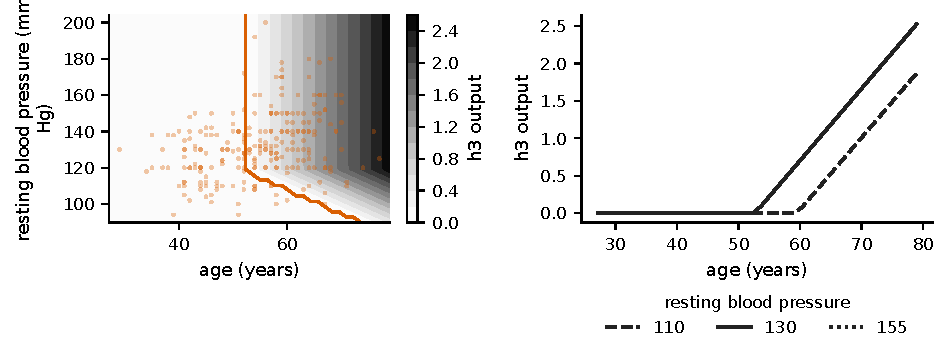
\includegraphics[width=\linewidth,height=0.88\textheight,keepaspectratio]{figures/heart-s5-c1/ann_34-partial-1987.pdf}
\caption{Extra age term: This part's own output, unit h3 (the output of 'Extra age term'), on its own scale (its activation), with every other input at the typical case; it is active for 85 of 242. Left: its output over its two main inputs (orange line: where it switches on; dots: the data); right: slices at three values of the second input.}
\label{fig:hearts5c1:plot-ann34-1}
\end{figure}
\begin{figure}[H]\centering
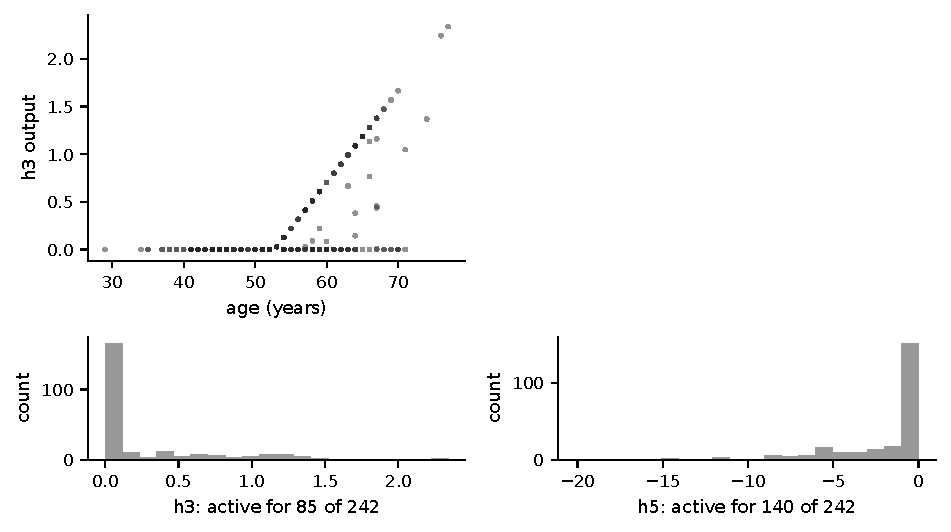
\includegraphics[width=\linewidth,height=0.88\textheight,keepaspectratio]{figures/heart-s5-c1/ann_34-units.pdf}
\caption{Extra age term: This part's hidden units: each unit's output against its main numeric input (top) and how often it is active (bottom).}
\label{fig:hearts5c1:plot-ann34-2}
\end{figure}
\par\smallskip\noindent{\small Technical detail: \ref{tech:ann34}.\par}
\subsection{Not supported by the model}
\begin{itemize}\setlength\itemsep{0pt}\small
\item C43: direction claim about resting blood pressure in part ann\_\allowbreak{}33: not supported by the model (17\% of patients have the opposite sign (allowed: 10\%)).
\item C45: interaction claim about resting blood pressure and chest pain type in part ann\_\allowbreak{}33: not supported by the model (the group difference is below 0.1 log-odds; the part's own counterfactual difference has the opposite sign).
\item C46: threshold claim about resting blood pressure in part ann\_\allowbreak{}33: not supported by the model (the effect past the fold is too small or not consistent across patients).
\item C47: subgroup claim about chest pain type and resting blood pressure in part ann\_\allowbreak{}33: not supported by the model (its effect goes both ways across the patients it acts on).
\end{itemize}
\clearpage\section*{Technical detail: heart-s5-c1}
\addcontentsline{toc}{section}{Technical detail: heart-s5-c1}
\noindent{\small The record behind each part: the original hypothesis, the closed form, and every claim with its estimate (log-odds and odds ratio), range across patients, n and test check.\par}
\renewcommand{\thesubsection}{T.\arabic{subsection}}\setcounter{subsection}{0}
\subsection{The whole model}\label{tech:ann35}
\noindent{\footnotesize Annotation ann\_\allowbreak{}35 (heart\_\allowbreak{}disease\_\allowbreak{}logit). Reads: age, sex, chest pain type, resting blood pressure, serum cholesterol, fasting blood sugar, resting ECG, maximum heart rate reached during the exercise test, exercise-induced angina, ST depression during exercise (compared with rest), slope of the ST segment at peak exercise, number of major vessels coloured by fluoroscopy, thallium stress test result.\par}
\paragraph{Original hypothesis (unchanged).} Root: p = sigmoid(z), z = -0.504 + LINEAR CORE + 0.143*ischaemia\_\allowbreak{}gate + 0.170*bp\_\allowbreak{}offset\_\allowbreak{}gate + 0.143*\allowbreak{}age\_\allowbreak{}gate\_\allowbreak{}without\_\allowbreak{}ischaemia. LINEAR CORE (19 direct input-$>$output edges, z-scored inputs): ca +1.480, sex:0 -1.072, slope:1 -0.855, chol +0.546, cp:1 -0.493, trestbps +0.480, cp:3 -0.440, exang:1 +0.431, thal:3 -0.410, thal:6 -0.384, cp:4 +0.377, slope:3 -0.366, fbs:0 +0.278, thalach -0.207, thal:4 +0.183, slope:2 +0.153, exang:0 +0.149, age +0.117, thal:7 -0.077. Four inputs are unconnected (sex:1, fbs:1, restecg:1, restecg:2; zero-effect entries of this root). Oldpeak, restecg:0 and cp:2 have no direct edge and act only through the chain. COMPOSITION: serial and additive. The three children form a chain, each read out additively into z: ischaemia\_\allowbreak{}gate (oldpeak, normal resting ECG, reversible defect) feeds bp\_\allowbreak{}offset\_\allowbreak{}gate (the ischaemia score minus a resting-BP offset), which in turn switches off age\_\allowbreak{}gate\_\allowbreak{}without\_\allowbreak{}ischaemia (an extra age term for patients without ischaemia evidence). The chain therefore raises risk with ST depression, more steeply where resting BP is low, and adds a small age term where the chain is quiet. Identity nodes identity\_\allowbreak{}290 and identity\_\allowbreak{}1987 carry the chain links (204 -$>$ 290, 290 -$>$ 1987) so that each gate is its own leaf. EVIDENCE (train, n=242): full model AUC 0.9418, acc 0.872 (compute\_\allowbreak{}performance)\allowbreak{}. Linear core alone AUC 0.934; logit SD 3.14 (core) vs 0.67 (chain). Removing the whole chain (node 204 with downstream) gives 0.934; readout-only ablations: ischaemia 0.940, BP 0.939, age 0.941. Treating all three ReLUs as identities gives 0.936; one least-squares linear fit of the chain on its seven inputs gives 0.937 (R2 0.84); an L2 logistic regression on all 26 inputs gives 0.936. Mean $|$SHAP$|$ (train, all 242): ca 0.144, sex:0 0.110, slope:1 0.100, thal:3 0.048, exang:1 0.047, chol 0.045, cp:4 0.044, cp:3 0.044. Interpretation: close to logistic regression plus one ischaemia correction: ST depression raises risk only above a threshold set by a normal resting ECG and a reversible defect, more so when resting BP is low; age gets a small extra weight when there is no such evidence. Counter-directional signs reported, not explained: restecg:0 positive in the ischaemia gate, trestbps negative in the BP gate, fbs:0 +0.28 directly. Same design as the 10-seed heart-s5 record (generation 37, key 9330: ischaemia gate -$>$ resting-BP gate -$>$ age term), here with three hidden nodes instead of six.
\paragraph{Closed form.} Read through its parts (their formulas are in their own sections).
\paragraph{Split inputs.} To annotate the parts, the explanation split these inputs into copies (a refactoring step that does not change what the model computes); the diagrams draw each input once: age (2 copies); non-anginal pain (2 copies); reversible defect (2 copies); blood pressure (2 copies).
\paragraph{Evidence table} (next page, landscape).
\begin{landscape}
{\scriptsize\setlength{\tabcolsep}{3pt}\renewcommand{\arraystretch}{1.15}
\rowcolors{2}{black!6}{white}
\begin{longtable}{@{}l>{\raggedright\arraybackslash}p{0.36\linewidth}>{\raggedright\arraybackslash}p{0.14\linewidth}rrr>{\raggedright\arraybackslash}p{0.06\linewidth}>{\raggedright\arraybackslash}p{0.17\linewidth}c@{}}
\toprule\rowcolor{white}
ID & What is checked & Risk, typical patient & Log-odds & OR & Range (p10--p90) & n & Test check & OK \\
\midrule\endfirsthead
\toprule\rowcolor{white}
ID & What is checked & Risk, typical patient & Log-odds & OR & Range (p10--p90) & n & Test check & OK \\
\midrule\endhead
\bottomrule\endfoot
C01 & direction: number of vessels coloured by fluoroscopy: 0 vessels to 2 vessels (whole model) \newline{\itshape shape: steady (equal steps); 100\% of patients same; verified; risk saturates near 100\%} & 22\% to 88\% & 3.32 & 27.6 & 3.32 to 3.32 & 242 & unclear; AUC gain 0.039 [-0.026, 0.111] & \textcolor{OliveGreen}{yes} \\
C02 & direction: thallium stress test result: a normal thallium scan to thallium stress test result coded 4 (meaning not recorded) (direct contribution only, not through any part) \newline{\itshape shape: categorical; highest to lowest: thallium stress test result coded 4 (meaning not recorded), a reversible defect on the thallium scan, a normal thallium scan, a fixed defect on the thallium scan} & 22\% to 83\% & 2.85 & 17.3 & 2.85 to 2.85 & 135, 2 (small n) & unclear; AUC gain 0.012 [-0.009, 0.035] & \textcolor{OliveGreen}{yes} \\
C03 & direction: thallium stress test result: a normal thallium scan to thallium stress test result coded 4 (meaning not recorded) (whole model) \newline{\itshape shape: categorical; highest to lowest: thallium stress test result coded 4 (meaning not recorded), a reversible defect on the thallium scan, a normal thallium scan, a fixed defect on the thallium scan} & 22\% to 83\% & 2.85 & 17.3 & 2.85 to 2.85 & 135, 2 (small n) & unclear; AUC gain 0.017 [-0.010, 0.052] & \textcolor{OliveGreen}{yes} \\
C04 & direction: slope of the ST segment at peak exercise: an upsloping ST segment to a flat ST segment (whole model) \newline{\itshape shape: categorical; highest to lowest: a flat ST segment, a downsloping ST segment, an upsloping ST segment} & 22\% to 67\% & 2.02 & 7.53 & 2.02 to 2.02 & 115, 110 & disagrees; AUC gain -0.019 [-0.070, 0.025] & \textcolor{OliveGreen}{yes} \\
C05 & direction: ST depression on exercise: 0.0 mm to 2.8 mm (whole model) \newline{\itshape shape: accelerating; 48\% of patients same; fallback} & 22\% to 48\% & 1.16 & 3.20 & 0.55 to 1.91 & 242 & unclear; AUC gain 0.008 [-0.011, 0.031] & \textcolor{OliveGreen}{yes} \\
C06 & direction: thallium stress test result: a normal thallium scan to a reversible defect on the thallium scan (whole model) \newline{\itshape shape: categorical; highest to lowest: thallium stress test result coded 4 (meaning not recorded), a reversible defect on the thallium scan, a normal thallium scan, a fixed defect on the thallium scan} & 22\% to 47\% & 1.01 & 2.73 & 0.67 to 1.44 & 135, 90 & unclear; AUC gain 0.017 [-0.010, 0.052] & \textcolor{OliveGreen}{yes} \\
C07 & direction: serum cholesterol: 193 mg/dL (5.0 mmol/L) to 308 mg/dL (8.0 mmol/L) (whole model) \newline{\itshape shape: steady; 100\% of patients same; verified} & 14\% to 37\% & 1.30 & 3.68 & 1.30 to 1.30 & 242 & disagrees; AUC gain -0.022 [-0.063, 0.008] & \textcolor{OliveGreen}{yes} \\
C08 & direction: resting blood pressure: 110 mm Hg to 155 mm Hg (direct contribution only, not through any part) \newline{\itshape shape: steady; 100\% of patients same; verified} & 14\% to 35\% & 1.19 & 3.28 & 1.19 to 1.19 & 242 & unclear; AUC gain 0.000 [-0.024, 0.022] & \textcolor{OliveGreen}{yes} \\
C09 & direction: resting blood pressure: 110 mm Hg to 155 mm Hg (whole model) \newline{\itshape shape: steady; 43\% of patients same; fallback} & 14\% to 35\% & 1.04 & 2.82 & 0.84 to 1.21 & 242 & unclear; AUC gain 0.001 [-0.022, 0.023] & \textcolor{OliveGreen}{yes} \\
C10 & direction: chest pain type: no chest pain (asymptomatic) to typical angina (direct contribution only, not through any part) \newline{\itshape shape: categorical; highest to lowest: no chest pain (asymptomatic), atypical angina, non-anginal chest pain, typical angina} & 22\% to 2\% & -2.48 & 0.08 & -2.48 to -2.48 & 108, 22 & agrees; AUC gain 0.040 [0.008, 0.079] & \textcolor{OliveGreen}{yes} \\
C11 & direction: chest pain type: no chest pain (asymptomatic) to typical angina (whole model) \newline{\itshape shape: categorical; highest to lowest: no chest pain (asymptomatic), atypical angina, non-anginal chest pain, typical angina} & 22\% to 2\% & -2.48 & 0.08 & -2.48 to -2.48 & 108, 22 & agrees; AUC gain 0.040 [0.008, 0.079] & \textcolor{OliveGreen}{yes} \\
C12 & direction: sex: male to female (whole model) \newline{\itshape shape: categorical; highest to lowest: male, female} & 22\% to 3\% & -2.26 & 0.10 & -2.26 to -2.26 & 159, 83 & unclear; AUC gain 0.024 [-0.008, 0.064] & \textcolor{OliveGreen}{yes} \\
C13 & direction: chest pain type: no chest pain (asymptomatic) to non-anginal chest pain (direct contribution only, not through any part) \newline{\itshape shape: categorical; highest to lowest: no chest pain (asymptomatic), atypical angina, non-anginal chest pain, typical angina} & 22\% to 5\% & -1.73 & 0.18 & -1.73 to -1.73 & 108, 70 & agrees; AUC gain 0.040 [0.008, 0.079] & \textcolor{OliveGreen}{yes} \\
C14 & direction: chest pain type: no chest pain (asymptomatic) to non-anginal chest pain (whole model) \newline{\itshape shape: categorical; highest to lowest: no chest pain (asymptomatic), atypical angina, non-anginal chest pain, typical angina} & 22\% to 5\% & -1.73 & 0.18 & -1.73 to -1.72 & 108, 70 & agrees; AUC gain 0.040 [0.008, 0.079] & \textcolor{OliveGreen}{yes} \\
C15 & direction: thallium stress test result: a normal thallium scan to a reversible defect on the thallium scan (direct contribution only, not through any part) \newline{\itshape shape: categorical; highest to lowest: thallium stress test result coded 4 (meaning not recorded), a reversible defect on the thallium scan, a normal thallium scan, a fixed defect on the thallium scan} & 22\% to 35\% & 0.67 & 1.95 & 0.67 to 0.67 & 135, 90 & unclear; AUC gain 0.012 [-0.009, 0.035] & \textcolor{OliveGreen}{yes} \\
C16 & direction: exercise-induced angina: no chest pain on exercise to chest pain brought on by exercise (whole model) \newline{\itshape shape: categorical; highest to lowest: chest pain brought on by exercise, no chest pain on exercise} & 22\% to 33\% & 0.60 & 1.82 & 0.60 to 0.60 & 160, 82 & unclear; AUC gain 0.012 [-0.003, 0.032] & \textcolor{OliveGreen}{yes} \\
C17 & direction: fasting blood sugar: fasting blood sugar of 120 mg/dL or less to fasting blood sugar above 120 mg/dL (whole model) \newline{\itshape shape: categorical; highest to lowest: fasting blood sugar of 120 mg/dL or less, fasting blood sugar above 120 mg/dL} & 22\% to 11\% & -0.81 & 0.44 & -0.81 to -0.81 & 209, 33 & disagrees; AUC gain -0.002 [-0.020, 0.015] & \textcolor{OliveGreen}{yes} \\
C18 & direction: thallium stress test result: a normal thallium scan to a fixed defect on the thallium scan (direct contribution only, not through any part) \newline{\itshape shape: categorical; highest to lowest: thallium stress test result coded 4 (meaning not recorded), a reversible defect on the thallium scan, a normal thallium scan, a fixed defect on the thallium scan} & 22\% to 11\% & -0.77 & 0.46 & -0.77 to -0.77 & 135, 15 (small n) & unclear; AUC gain 0.012 [-0.009, 0.035] & \textcolor{OliveGreen}{yes} \\
C19 & direction: thallium stress test result: a normal thallium scan to a fixed defect on the thallium scan (whole model) \newline{\itshape shape: categorical; highest to lowest: thallium stress test result coded 4 (meaning not recorded), a reversible defect on the thallium scan, a normal thallium scan, a fixed defect on the thallium scan} & 22\% to 11\% & -0.77 & 0.46 & -0.77 to -0.77 & 135, 15 (small n) & unclear; AUC gain 0.017 [-0.010, 0.052] & \textcolor{OliveGreen}{yes} \\
C20 & direction: chest pain type: no chest pain (asymptomatic) to atypical angina (direct contribution only, not through any part) \newline{\itshape shape: categorical; highest to lowest: no chest pain (asymptomatic), atypical angina, non-anginal chest pain, typical angina} & 22\% to 11\% & -0.76 & 0.47 & -0.76 to -0.76 & 108, 42 & agrees; AUC gain 0.040 [0.008, 0.079] & \textcolor{OliveGreen}{yes} \\
C21 & direction: chest pain type: no chest pain (asymptomatic) to atypical angina (whole model) \newline{\itshape shape: categorical; highest to lowest: no chest pain (asymptomatic), atypical angina, non-anginal chest pain, typical angina} & 22\% to 11\% & -0.72 & 0.49 & -0.76 to -0.68 & 108, 42 & agrees; AUC gain 0.040 [0.008, 0.079] & \textcolor{OliveGreen}{yes} \\
C22 & direction: maximum heart rate: 118 beats per minute to 175 beats per minute (whole model) \newline{\itshape shape: steady; 100\% of patients same; verified} & 27\% to 18\% & -0.53 & 0.59 & -0.53 to -0.53 & 242 & unclear; AUC gain 0.006 [0.000, 0.022] & \textcolor{OliveGreen}{yes} \\
C23 & direction: age: 42 years to 66 years (whole model) \newline{\itshape shape: accelerating; 67\% of patients same; fallback} & 18\% to 26\% & 0.41 & 1.50 & 0.31 to 0.49 & 242 & disagrees; AUC gain -0.003 [-0.017, 0.013] & \textcolor{OliveGreen}{yes} \\
C24 & direction: age: 42 years to 66 years (direct contribution only, not through any part) \newline{\itshape shape: steady; 100\% of patients same; verified} & 19\% to 24\% & 0.31 & 1.36 & 0.31 to 0.31 & 242 & disagrees; AUC gain -0.004 [-0.018, 0.012] & \textcolor{OliveGreen}{yes} \\
C25 & direction: slope of the ST segment at peak exercise: an upsloping ST segment to a downsloping ST segment (whole model) \newline{\itshape shape: categorical; highest to lowest: a flat ST segment, a downsloping ST segment, an upsloping ST segment} & 22\% to 27\% & 0.28 & 1.32 & 0.28 to 0.28 & 115, 17 (small n) & disagrees; AUC gain -0.019 [-0.070, 0.025] & \textcolor{OliveGreen}{yes} \\
C26 & direction: resting ECG: a normal resting ECG to resting ECG other than a normal resting ECG (whole model) \newline{\itshape shape: categorical; highest to lowest: a normal resting ECG, resting ECG other than a normal resting ECG} & 22\% to 22\% & -0.23 & 0.80 & -0.57 to 0.00 & 121, 121 & disagrees; AUC gain -0.002 [-0.015, 0.009] & \textcolor{OliveGreen}{yes} \\
C27 & magnitude: number of vessels coloured by fluoroscopy: 0 vessels to 2 vessels, typical patient \newline{\itshape shape: steady (equal steps); 100\% of patients same; verified; risk saturates near 100\%} & 22\% to 88\% & 3.32 & 27.6 &  & 242 & unclear; AUC gain 0.039 [-0.026, 0.111] & \textcolor{OliveGreen}{yes} \\
C28 & magnitude: slope of the ST segment at peak exercise: an upsloping ST segment to a flat ST segment, typical patient \newline{\itshape shape: categorical; highest to lowest: a flat ST segment, a downsloping ST segment, an upsloping ST segment} & 22\% to 67\% & 2.02 & 7.53 &  & 115, 110 & disagrees; AUC gain -0.019 [-0.070, 0.025] & \textcolor{OliveGreen}{yes} \\
C29 & magnitude: ST depression on exercise: 0.0 mm to 2.8 mm, typical patient \newline{\itshape shape: accelerating; 48\% of patients same; fallback} & 22\% to 48\% & 1.21 & 3.36 &  & 242 & unclear; AUC gain 0.008 [-0.011, 0.031] & \textcolor{OliveGreen}{yes} \\
C30 & magnitude: thallium stress test result: a normal thallium scan to a reversible defect on the thallium scan, typical patient \newline{\itshape shape: categorical; highest to lowest: thallium stress test result coded 4 (meaning not recorded), a reversible defect on the thallium scan, a normal thallium scan, a fixed defect on the thallium scan} & 22\% to 47\% & 1.19 & 3.28 &  & 135, 90 & unclear; AUC gain 0.017 [-0.010, 0.052] & \textcolor{OliveGreen}{yes} \\
C31 & magnitude: serum cholesterol: 193 mg/dL (5.0 mmol/L) to 308 mg/dL (8.0 mmol/L), typical patient \newline{\itshape shape: steady; 100\% of patients same; verified} & 14\% to 37\% & 1.30 & 3.68 &  & 242 & disagrees; AUC gain -0.022 [-0.063, 0.008] & \textcolor{OliveGreen}{yes} \\
C32 & structure: made of ischaemia\_\allowbreak{}gate, bp\_\allowbreak{}offset\_\allowbreak{}gate, age\_\allowbreak{}gate\_\allowbreak{}without\_\allowbreak{}ischaemia and inputs age, sex, cp, trestbps, chol, fbs, thalach, exang, slope, ca, thal; added; ann\_\allowbreak{}32 feeds ann\_\allowbreak{}33; ann\_\allowbreak{}33 feeds ann\_\allowbreak{}34 &  &  &  &  & 242 & train only & \textcolor{OliveGreen}{yes} \\
\end{longtable}}
\end{landscape}
\subsection{ST depression and thallium signal}\label{tech:ann32}
\noindent{\footnotesize Annotation ann\_\allowbreak{}32 (ischaemia\_\allowbreak{}gate). Reads: resting ECG, ST depression during exercise (compared with rest), thallium stress test result.\par}
\paragraph{Original hypothesis (unchanged).} Ischaemia-evidence gate (raises risk). 204 = ReLU(0.247 + 2.593*oldpeak + 0.871*restecg:0 + 1.145*thal:7). Hypothesis: a one-sided ST-depression score that opens above an oldpeak threshold set by two flags (always open with a normal resting ECG and a reversible thallium defect; above z-oldpeak -0.09 with a normal ECG only, -0.33 with a defect only, +0.58 with neither), and then raises the logit with oldpeak, directly (0.143 per unit) and through the blood-pressure gate (a further 0.183 per unit while that gate is open). EVIDENCE (train, n=242): active for 48\% (100\% of the 44 patients with both flags, 20\% of the 75 with neither); corr with oldpeak 0.88; disease rate 66\% when active vs 24\% when inactive. Mean $|$sensitivity$|$ oldpeak 1.24 $>$ thal:7 0.55 $>$ restecg:0 0.42. This is the main nonlinear effect: removing it with its downstream effects lowers train AUC 0.942 -$>$ 0.934 (to the linear-core level); an affine replacement recovers 0.938. Supported. Oldpeak and restecg:0 have no direct edge; they act only here. The positive restecg:0 weight (normal ECG raises the score) is counter-intuitive and is reported, not explained.
\paragraph{Closed form} {\footnotesize(weights and biases at 3 significant figures; largest difference from the part on the training patients 1.77636e-15).}
{\small\begingroup\allowdisplaybreaks
\begin{align*}
y_{0} &= \operatorname{relu}\bigl(0.247 + 1.15 x_{thal:7\_b} + 2.59 x_{oldpeak} \\
&\qquad + 0.87 x_{restecg:0}\bigr)
\end{align*}\endgroup}

\paragraph{Evidence table} (next page, landscape).
\begin{landscape}
{\scriptsize\setlength{\tabcolsep}{3pt}\renewcommand{\arraystretch}{1.15}
\rowcolors{2}{black!6}{white}
\begin{longtable}{@{}l>{\raggedright\arraybackslash}p{0.36\linewidth}>{\raggedright\arraybackslash}p{0.14\linewidth}rrr>{\raggedright\arraybackslash}p{0.06\linewidth}>{\raggedright\arraybackslash}p{0.17\linewidth}c@{}}
\toprule\rowcolor{white}
ID & What is checked & Risk, typical patient & Log-odds & OR & Range (p10--p90) & n & Test check & OK \\
\midrule\endfirsthead
\toprule\rowcolor{white}
ID & What is checked & Risk, typical patient & Log-odds & OR & Range (p10--p90) & n & Test check & OK \\
\midrule\endhead
\bottomrule\endfoot
C33 & direction: ST depression on exercise: 0.0 mm to 2.8 mm (through this part) \newline{\itshape shape: accelerating; 48\% of patients same; fallback} & 22\% to 48\% & 1.16 & 3.20 & 0.55 to 1.91 & 242 & unclear; AUC gain 0.008 [-0.011, 0.031] & \textcolor{OliveGreen}{yes} \\
C34 & direction: thallium stress test result: thallium stress test result other than a reversible defect on the thallium scan to a reversible defect on the thallium scan (through this part) \newline{\itshape shape: categorical; highest to lowest: a reversible defect on the thallium scan, thallium stress test result other than a reversible defect on the thallium scan} & 22\% to 32\% & 0.34 & 1.40 & 0.00 to 0.77 & 152, 90 & unclear; AUC gain 0.005 [-0.009, 0.025] & \textcolor{OliveGreen}{yes} \\
C35 & direction: resting ECG: a normal resting ECG to resting ECG other than a normal resting ECG (through this part) \newline{\itshape shape: categorical; highest to lowest: a normal resting ECG, resting ECG other than a normal resting ECG} & 96\% to 94\% (typical patient this part acts on) & -0.23 & 0.80 & -0.57 to 0.00 & 121, 121 & disagrees; AUC gain -0.002 [-0.015, 0.009] & \textcolor{OliveGreen}{yes} \\
C36 & interaction: effect of ST depression on exercise (0.0 mm to 2.8 mm) by thallium stress test result: a reversible defect on the thallium scan minus thallium stress test result other than a reversible defect on the thallium scan; stronger in a reversible defect on the thallium scan \newline{\itshape shape: steady; 37\% of patients same; fallback} & a reversible defect on the thallium scan: 36\% to 80\%; thallium stress test result other than a reversible defect on the thallium scan: 22\% to 48\% & 0.68 & 1.98 &  & 90, 152 & agrees; AUC gain 0.005 [-0.009, 0.025] & \textcolor{OliveGreen}{yes} \\
C37 & interaction: effect of ST depression on exercise (0.0 mm to 2.8 mm) by resting ECG: resting ECG other than a normal resting ECG minus a normal resting ECG; stronger in a normal resting ECG \newline{\itshape shape: accelerating; 33\% of patients same; fallback} & resting ECG other than a normal resting ECG: 22\% to 34\%; a normal resting ECG: 22\% to 48\% & -0.59 & 0.55 &  & 121, 121 & agrees; AUC gain -0.002 [-0.015, 0.009] & \textcolor{OliveGreen}{yes} \\
C38 & interaction: effect of thallium stress test result (thallium stress test result other than a reversible defect on the thallium scan to a reversible defect on the thallium scan) by resting ECG: resting ECG other than a normal resting ECG minus a normal resting ECG; stronger in a normal resting ECG \newline{\itshape shape: categorical; highest to lowest: a reversible defect on the thallium scan, thallium stress test result other than a reversible defect on the thallium scan} & resting ECG other than a normal resting ECG: 22\% to 36\%; a normal resting ECG: 22\% to 47\% & -0.11 & 0.90 &  & 121, 121 & agrees; AUC gain -0.002 [-0.015, 0.009] & \textcolor{OliveGreen}{yes} \\
C39 & threshold: ST depression on exercise: fold at about 0.9 mm (starts) \newline{\itshape shape: accelerating; 55\% of patients same; fallback} & 22\% to 46\% (typical patient with a fold) & 1.50 & 4.47 & 1.00 to 1.86 & 198, 72 & unclear; AUC gain 0.008 [-0.011, 0.031] & \textcolor{OliveGreen}{yes} \\
C40 & subgroup: who this part acts on: 116 of 242 patients & 89\% to 96\% (typical patient this part acts on (risk without the part, then with it)) & 0.77 & 2.17 & 0.08 to 1.75 & 116, 126 & unclear; AUC gain 0.016 [-0.005, 0.048] & \textcolor{OliveGreen}{yes} \\
C41 & structure: its formula reproduces it on 242 training patients (largest difference 1.77636e-15) &  & 2e-15 &  &  & 242 & train only & \textcolor{OliveGreen}{yes} \\
\end{longtable}}
\end{landscape}
\subsection{Blood pressure step}\label{tech:ann33}
\noindent{\footnotesize Annotation ann\_\allowbreak{}33 (bp\_\allowbreak{}offset\_\allowbreak{}gate). Reads: chest pain type, resting blood pressure.\par}
\paragraph{Original hypothesis (unchanged).} Blood-pressure offset gate on the ischaemia score (raises risk). 290 = ReLU(-0.495 + 1.079*ischaemia\_\allowbreak{}gate - 0.815*trestbps + 0.176*cp:2 + 0.016*cp:3). Hypothesis: passes the ischaemia score on, minus an offset that grows with resting blood pressure; it adds 0.170 per unit to the logit and switches off the age gate. With the ischaemia gate closed it still opens for low resting blood pressure, so within this gate lower resting BP raises risk (0.170*0.815 = 0.139 per SD), partly offsetting trestbps's direct +0.48 edge. cp:2 (atypical angina) nudges it open; cp:3's weight 0.016 is negligible. EVIDENCE (train, n=242): active for 58\% (83\% with the ischaemia gate open, 35\% without); with the ischaemia gate open, active for 100\%, 87\% and 59\% of the low, middle and high resting-BP groups. Disease rate 51\% when active vs 35\% when inactive. Mean $|$sensitivity$|$ ischaemia score 0.58 $>$ trestbps 0.45 $>$ cp:2 0.10 $>$ cp:3 0.01. Readout ablation lowers train AUC 0.942 -$>$ 0.939; an affine replacement fits it well (R2 0.97, AUC 0.941), so its nonlinearity matters little. Supported, small. The negative BP term inside a risk-raising gate is reported, not explained.
\paragraph{Closed form} {\footnotesize(weights and biases at 3 significant figures; largest difference from the part on the training patients 8.88178e-16).}
{\small\begingroup\allowdisplaybreaks
\begin{align*}
y_{0} &= \operatorname{relu}\bigl(-0.495 + 1.0 x_{identity\_290} + 0.0164 x_{cp:3\_b} \\
&\qquad + 0.176 x_{cp:2} - 0.815 x_{trestbps\_b}\bigr)
\end{align*}\endgroup}

\paragraph{Evidence table} (next page, landscape).
\begin{landscape}
{\scriptsize\setlength{\tabcolsep}{3pt}\renewcommand{\arraystretch}{1.15}
\rowcolors{2}{black!6}{white}
\begin{longtable}{@{}l>{\raggedright\arraybackslash}p{0.36\linewidth}>{\raggedright\arraybackslash}p{0.14\linewidth}rrr>{\raggedright\arraybackslash}p{0.06\linewidth}>{\raggedright\arraybackslash}p{0.17\linewidth}c@{}}
\toprule\rowcolor{white}
ID & What is checked & Risk, typical patient & Log-odds & OR & Range (p10--p90) & n & Test check & OK \\
\midrule\endfirsthead
\toprule\rowcolor{white}
ID & What is checked & Risk, typical patient & Log-odds & OR & Range (p10--p90) & n & Test check & OK \\
\midrule\endhead
\bottomrule\endfoot
C42 & direction: chest pain type: chest pain type other than atypical angina, non-anginal chest pain to atypical angina (through this part) \newline{\itshape shape: categorical; highest to lowest: atypical angina, non-anginal chest pain, chest pain type other than atypical angina, non-anginal chest pain} & 69\% to 70\% (typical patient this part acts on) & 0.04 & 1.04 & 0.00 to 0.08 & 130, 42 & unclear; AUC gain 0.000 [0.000, 0.000] & \textcolor{OliveGreen}{yes} \\
C43 & direction: resting blood pressure: 110 mm Hg to 155 mm Hg (through this part) \newline{\itshape shape: hinge at 114 mm Hg; 45\% of patients same; fallback} & 22\% to 22\% & -0.15 & 0.86 & -0.34 to 0.02 & 242 & disagrees; AUC gain -0.003 [-0.015, 0.006] & \textcolor{BrickRed}{no} \\
C44 & direction: chest pain type: chest pain type other than atypical angina, non-anginal chest pain to non-anginal chest pain (through this part) \newline{\itshape shape: categorical; highest to lowest: atypical angina, non-anginal chest pain, chest pain type other than atypical angina, non-anginal chest pain} & 69\% to 69\% (typical patient this part acts on) & 0.003 & 1.00 & 0.00 to 0.006 & 130, 70 & unclear; AUC gain 0.000 [0.000, 0.000] & \textcolor{OliveGreen}{yes} \\
C45 & interaction: effect of resting blood pressure (110 mm Hg to 155 mm Hg) by chest pain type: atypical angina minus chest pain type other than atypical angina, non-anginal chest pain; stronger in atypical angina \newline{\itshape shape: accelerating; 90\% of patients same; verified} & atypical angina: 8\% to 20\%; chest pain type other than atypical angina, non-anginal chest pain: 14\% to 35\% & 0.04 & 1.04 &  & 42, 130 & unclear; AUC gain 0.000 [0.000, 0.000] & \textcolor{BrickRed}{no} \\
C46 & threshold: resting blood pressure: fold at about 128 mm Hg (stops) \newline{\itshape shape: several pieces; 14\% of patients same; fallback} & 22\% to 21\% (typical patient with a fold) & -0.16 & 0.85 & -0.42 to 0.03 & 203, 101 & disagrees; AUC gain -0.003 [-0.015, 0.006] & \textcolor{BrickRed}{no} \\
C47 & subgroup: who this part acts on: 140 of 242 patients & 65\% to 69\% (typical patient this part acts on (risk without the part, then with it)) & 0.33 & 1.39 & -0.01 to 0.84 & 140, 102 & unclear; AUC gain 0.006 [-0.004, 0.022] & \textcolor{BrickRed}{no} \\
C48 & structure: its formula reproduces it on 242 training patients (largest difference 8.88178e-16) &  & 9e-16 &  &  & 242 & train only & \textcolor{OliveGreen}{yes} \\
\end{longtable}}
\end{landscape}
\subsection{Extra age term}\label{tech:ann34}
\noindent{\footnotesize Annotation ann\_\allowbreak{}34 (age\_\allowbreak{}gate\_\allowbreak{}without\_\allowbreak{}ischaemia). Reads: age.\par}
\paragraph{Original hypothesis (unchanged).} Age gate without ischaemia evidence (raises risk with age, small). 1987 = ReLU(0.203 + 0.875*age - 1.589*\allowbreak{}bp\_\allowbreak{}offset\_\allowbreak{}gate)\allowbreak{},\allowbreak{} read out +0.143. Hypothesis: an extra age term (0.125 per SD of age, on top of age's direct +0.117) that acts only while the BP gate is closed or nearly closed, i.e. for patients without much ischaemia evidence; any opening of the BP gate cancels it (each unit of the BP gate removes 0.227 from the logit through this node until it closes). EVIDENCE (train, n=242): active for 35\% (65\% when the BP gate is closed, rising with age: 0\%, 80\%, 100\% of the youngest, middle and oldest groups; 14\% when the BP gate is open). Disease rate barely differs (43\% vs 45\%). Mean $|$sensitivity$|$ BP gate 0.35, age 0.31. Removing it lowers train AUC only 0.942 -$>$ 0.941. Supported, near-negligible.
\paragraph{Closed form} {\footnotesize(weights and biases at 3 significant figures; largest difference from the part on the training patients 1.11022e-16).}
{\small\begingroup\allowdisplaybreaks
\begin{align*}
y_{0} &= \operatorname{relu}\bigl(0.203 + 1.0 x_{identity\_1987} + 0.875 x_{age\_b}\bigr)
\end{align*}\endgroup}

\paragraph{Evidence table} (next page, landscape).
\begin{landscape}
{\scriptsize\setlength{\tabcolsep}{3pt}\renewcommand{\arraystretch}{1.15}
\rowcolors{2}{black!6}{white}
\begin{longtable}{@{}l>{\raggedright\arraybackslash}p{0.36\linewidth}>{\raggedright\arraybackslash}p{0.14\linewidth}rrr>{\raggedright\arraybackslash}p{0.06\linewidth}>{\raggedright\arraybackslash}p{0.17\linewidth}c@{}}
\toprule\rowcolor{white}
ID & What is checked & Risk, typical patient & Log-odds & OR & Range (p10--p90) & n & Test check & OK \\
\midrule\endfirsthead
\toprule\rowcolor{white}
ID & What is checked & Risk, typical patient & Log-odds & OR & Range (p10--p90) & n & Test check & OK \\
\midrule\endhead
\bottomrule\endfoot
C49 & direction: age: 42 years to 66 years (through this part) \newline{\itshape shape: hinge at 53 years; 99\% of patients same; verified; one point with C50 (median fold 53 years, typical patient 53 years, 10th-90th percentile 53 years to 66 years, wide)} & 21\% to 24\% & 0.10 & 1.11 & 0.00 to 0.18 & 242 & unclear; AUC gain 0.000 [-0.01, 0.011] & \textcolor{OliveGreen}{yes} \\
C50 & threshold: age: fold at about 53 years (starts) \newline{\itshape shape: hinge at 53 years; 99\% of patients same; verified; one point with C50 (median fold 53 years, typical patient 53 years, 10th-90th percentile 53 years to 66 years, wide)} & 20\% to 24\% (typical patient with a fold) & 0.17 & 1.18 & 0.03 to 0.21 & 174, 85 & unclear; AUC gain 0.000 [-0.01, 0.011] & \textcolor{OliveGreen}{yes} \\
C51 & subgroup: who this part acts on: 85 of 242 patients & 28\% to 30\% (typical patient this part acts on (risk without the part, then with it)) & 0.10 & 1.11 & 0.01 to 0.20 & 85, 157 & disagrees; AUC gain -0.002 [-0.01, 0.004] & \textcolor{OliveGreen}{yes} \\
C52 & structure: its formula reproduces it on 242 training patients (largest difference 1.11022e-16) &  & 1e-16 &  &  & 242 & train only & \textcolor{OliveGreen}{yes} \\
\end{longtable}}
\end{landscape}
\subsection*{The network before any explanation}\addcontentsline{toc}{subsection}{The network before any explanation} Figure~\ref{fig:hearts5c1:raw} (next page, landscape) is the trained network as it is, with no parts, no splits and no inserted units: inputs at the bottom, hidden units by depth, the output at the top, every connection drawn, every input column its own node (one-hot levels included).
\begin{landscape}
\begin{figure}[p]\centering
\resizebox{\linewidth}{!}{%
\definecolor{netup}{HTML}{D95F02}\definecolor{netdown}{HTML}{1B9E77}\definecolor{netmixed}{HTML}{7F7F7F}%
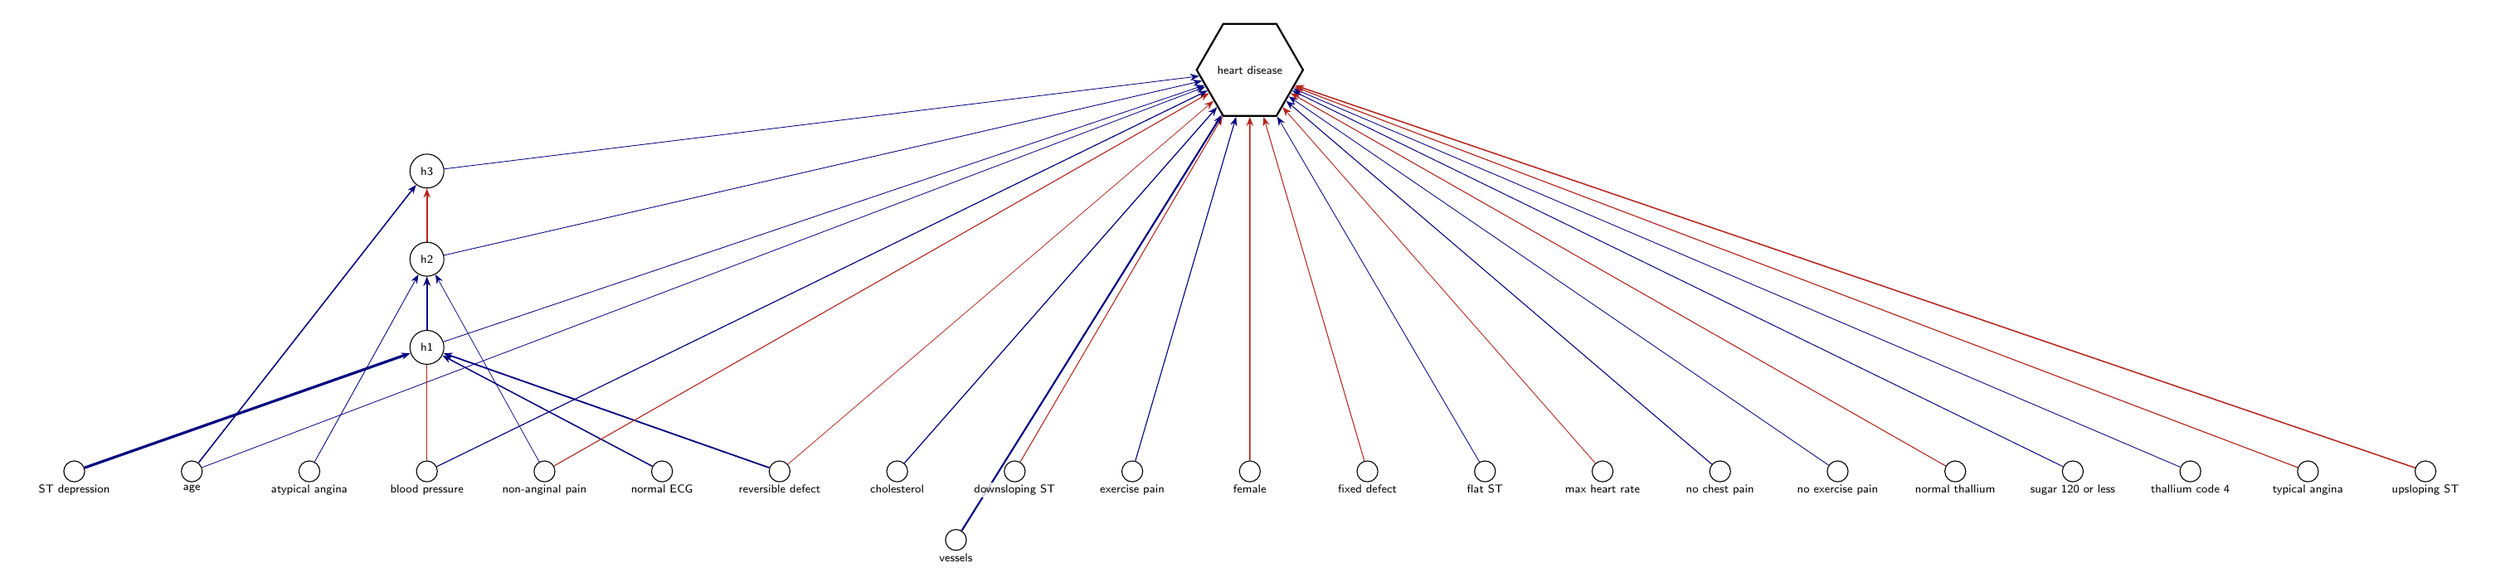
\begin{tikzpicture}[
  font=\sffamily\scriptsize, >={Stealth[length=1.4mm]},
  inp/.style={draw, circle, fill=white, minimum size=3.2mm, inner sep=0pt},
  hid/.style={draw, circle, fill=white, minimum size=5.2mm, inner sep=0.5pt, font=\sffamily\tiny},
  exitbox/.style={draw, thick, rectangle, fill=white, align=center, text width=17mm, minimum height=5mm, inner sep=1.5pt, font=\sffamily\tiny},
  sumbox/.style={draw, thick, dashed, rectangle, fill=white, align=center, text width=17mm, minimum height=5mm, inner sep=1.5pt, font=\sffamily\tiny},
  outp/.style={draw, thick, regular polygon, regular polygon sides=6, fill=white, minimum size=10mm, inner sep=0pt, font=\sffamily\tiny, align=center},
  stub/.style={draw, dashed, rounded corners=2pt, fill=white, align=center, inner sep=2pt, font=\sffamily\tiny, text width=15mm},
  inlab/.style={font=\sffamily\tiny, align=center, text width=15mm, inner sep=1pt, fill=white, fill opacity=0.8, text opacity=1},
  wpos/.style={draw=NavyBlue}, wneg/.style={draw=BrickRed}, wagg/.style={draw=black!45, line width=1.2pt},
  wmix/.style={draw=Plum},
]
\node[inp] (ninxxfbsx0) at (30.6,0.0) {};
\path (ninxxfbsx0.south) node[inlab, anchor=north] (labninxxfbsx0) {sugar 120 or less};
\node[inp] (ninxxrestecgx0) at (9.0,0.0) {};
\path (ninxxrestecgx0.south) node[inlab, anchor=north] (labninxxrestecgx0) {normal ECG};
\node[inp] (ninxxthalach) at (23.4,0.0) {};
\path (ninxxthalach.south) node[inlab, anchor=north] (labninxxthalach) {max heart rate};
\node[inp] (ninxxexangx0) at (27.0,0.0) {};
\path (ninxxexangx0.south) node[inlab, anchor=north] (labninxxexangx0) {no exercise pain};
\node[inp] (ninxxexangx1) at (16.2,0.0) {};
\path (ninxxexangx1.south) node[inlab, anchor=north] (labninxxexangx1) {exercise pain};
\node[inp] (ninxxoldpeak) at (0.0,0.0) {};
\path (ninxxoldpeak.south) node[inlab, anchor=north] (labninxxoldpeak) {ST depression};
\node[inp] (ninxxslopex1) at (36.0,0.0) {};
\path (ninxxslopex1.south) node[inlab, anchor=north] (labninxxslopex1) {upsloping ST};
\node[inp] (ninxxage) at (1.8,0.0) {};
\path (ninxxage.south) node[inlab, anchor=north] (labninxxage) {age};
\node[inp] (ninxxsexx0) at (18.0,0.0) {};
\path (ninxxsexx0.south) node[inlab, anchor=north] (labninxxsexx0) {female};
\node[inp] (ninxxslopex2) at (21.6,0.0) {};
\path (ninxxslopex2.south) node[inlab, anchor=north] (labninxxslopex2) {flat ST};
\node[inp] (ninxxslopex3) at (14.4,0.0) {};
\path (ninxxslopex3.south) node[inlab, anchor=north] (labninxxslopex3) {downsloping ST};
\node[inp] (ninxxca) at (13.5,-1.05) {};
\path (ninxxca.south) node[inlab, anchor=north] (labninxxca) {vessels};
\node[inp] (ninxxthalx3) at (28.8,0.0) {};
\path (ninxxthalx3.south) node[inlab, anchor=north] (labninxxthalx3) {normal thallium};
\node[inp] (ninxxthalx4) at (32.4,0.0) {};
\path (ninxxthalx4.south) node[inlab, anchor=north] (labninxxthalx4) {thallium code 4};
\node[inp] (ninxxthalx6) at (19.8,0.0) {};
\path (ninxxthalx6.south) node[inlab, anchor=north] (labninxxthalx6) {fixed defect};
\node[inp] (ninxxthalx7) at (10.8,0.0) {};
\path (ninxxthalx7.south) node[inlab, anchor=north] (labninxxthalx7) {reversible defect};
\node[inp] (ninxxcpx1) at (34.2,0.0) {};
\path (ninxxcpx1.south) node[inlab, anchor=north] (labninxxcpx1) {typical angina};
\node[inp] (ninxxcpx2) at (3.6,0.0) {};
\path (ninxxcpx2.south) node[inlab, anchor=north] (labninxxcpx2) {atypical angina};
\node[inp] (ninxxcpx3) at (7.2,0.0) {};
\path (ninxxcpx3.south) node[inlab, anchor=north] (labninxxcpx3) {non-anginal pain};
\node[inp] (ninxxcpx4) at (25.2,0.0) {};
\path (ninxxcpx4.south) node[inlab, anchor=north] (labninxxcpx4) {no chest pain};
\node[inp] (ninxxtrestbps) at (5.4,0.0) {};
\path (ninxxtrestbps.south) node[inlab, anchor=north] (labninxxtrestbps) {blood pressure};
\node[inp] (ninxxchol) at (12.6,0.0) {};
\path (ninxxchol.south) node[inlab, anchor=north] (labninxxchol) {cholesterol};
\node[outp] (n0) at (18.0,6.15) {heart disease};
\node[hid] (n1987) at (5.4,4.6) {h3};
\node[hid] (n204) at (5.4,1.9) {h1};
\node[hid] (n290) at (5.4,3.25) {h2};
\begin{scope}[on background layer]
\draw[->, wpos, line width=0.29pt] (ninxxage) -- (n0);
\draw[->, wpos, line width=0.56pt] (ninxxage) -- (n1987);
\draw[->, wpos, line width=0.35pt] (ninxxfbsx0) -- (n0);
\draw[->, wpos, line width=0.55pt] (ninxxrestecgx0) -- (n204);
\draw[->, wneg, line width=0.32pt] (ninxxthalach) -- (n0);
\draw[->, wpos, line width=0.30pt] (ninxxexangx0) -- (n0);
\draw[->, wpos, line width=0.40pt] (ninxxexangx1) -- (n0);
\draw[->, wpos, line width=1.16pt] (ninxxoldpeak) -- (n204);
\draw[->, wneg, line width=0.55pt] (ninxxslopex1) -- (n0);
\draw[->, wneg, line width=0.63pt] (ninxxsexx0) -- (n0);
\draw[->, wpos, line width=0.30pt] (ninxxslopex2) -- (n0);
\draw[->, wneg, line width=0.38pt] (ninxxslopex3) -- (n0);
\draw[->, wpos, line width=0.77pt] (ninxxca) -- (n0);
\draw[->, wneg, line width=0.39pt] (ninxxthalx3) -- (n0);
\draw[->, wpos, line width=0.31pt] (ninxxthalx4) -- (n0);
\draw[->, wneg, line width=0.38pt] (ninxxthalx6) -- (n0);
\draw[->, wneg, line width=0.28pt] (ninxxthalx7) -- (n0);
\draw[->, wpos, line width=0.65pt] (ninxxthalx7) -- (n204);
\draw[->, wneg, line width=0.42pt] (ninxxcpx1) -- (n0);
\draw[->, wpos, line width=0.31pt] (ninxxcpx2) -- (n290);
\draw[->, wneg, line width=0.40pt] (ninxxcpx3) -- (n0);
\draw[->, wpos, line width=0.26pt] (ninxxcpx3) -- (n290);
\draw[->, wpos, line width=0.38pt] (ninxxcpx4) -- (n0);
\draw[->, wpos, line width=0.42pt] (ninxxtrestbps) -- (n0);
\draw[->, wneg, line width=0.54pt] (ninxxtrestbps) -- (n290);
\draw[->, wpos, line width=0.44pt] (ninxxchol) -- (n0);
\draw[->, wpos, line width=0.30pt] (n1987) -- (n0);
\draw[->, wpos, line width=0.30pt] (n204) -- (n0);
\draw[->, wpos, line width=0.63pt] (n204) -- (n290);
\draw[->, wpos, line width=0.31pt] (n290) -- (n0);
\draw[->, wneg, line width=0.81pt] (n290) -- (n1987);
\end{scope}
\end{tikzpicture}}%
\caption{The network as trained, before any explanation, in full. Blue: positive weight (raises the score); red: negative weight (lowers it); thicker: larger weight. Orange outline and up arrow: raises the final prediction; teal and down arrow: lowers it; grey and double arrow: depends. Not used (no connection): male, sugar above 120, ST-T abnormal ECG, LVH on ECG.}
\label{fig:hearts5c1:raw}
\end{figure}
\end{landscape}
\end{drafted}
\clearpage
\end{document}
